This section describes the algorithm introduced in Ref.~\cite{harvardAlg} and its performance.
It also includes details of its implementation on an evaluation board and measurements performed
using that setup, as well as recent studies of the impact of
misalignments on the algorithm performance.



%Note:   Trigger algorithm design and performance can be found in the note An Algorithm for Micromegas Segment Reconstruction in the Level-1Trigger of the New Small Wheels by Brian Clark et al., resident in CDS: https://cds.cern.ch/record/1706160

%%%%%%%%% Sample inclusion of a figure
 % \begin{figure}[h]
 % \begin{center}
 % \includegraphics[width=0.8\textwidth]{algorithms-harvard/Plot1}
 % \caption{Caption of plot 1}
 % \label{fig:Monitoring}
 % \end{center}
 % \end{figure}

\subsubsubsection{Description}
This algorithm has been described in detail in Ref.\,\cite{harvardAlg}. Here, its main features are
summarized. The algorithm has four functionally distinct sets of operations:
\begin{enumerate}\itemsep-5pt
\item translation of hardware addresses into equivalent track slopes fixed to the IP,
\item determination of the presence of a multi-plane coincidence,
\item parallel calculation of global $\theta$ (azimuth of the track position at the entrance of the NSW)
and local $\theta$ (direction, at the entrance of the NSW, referred to as $\theta_{rec}$ in Section~\ref{sec:algorithms-saclay}) 
angles with parallel strips and global average stereo strips, 
using the multi-plane coincidence,
\item calculation of $\Delta\theta$, global $\theta$ (referred to as $\theta$ in what follows) and $\phi$.
\end{enumerate}
The first two items are performed by many {\em finders}, which don't consume significant amount
of resources, but reduce significantly the throughput towards the second half of the algorithm. Items
3 and 4 are performed by {\em fitters} that consume most of the resources allocated to the algorithm,
but only performed upon the presence of a solid track candidate.
Figure\,\ref{fig:harvardAlg} shows the algorithmic flow with smaller functional units. They are labeled
for easy reference when discussing the algorithm implementation.
	\begin{figure}[htbp]
	\begin{center}
	\includegraphics[width=\textwidth]{algorithms-harvard/block_detailed_V02.pdf}
	\caption{\label{fig:harvardAlg} The block diagram is constructed with time flowing downward; therefore tasks on the same horizontal line are accomplished in parallel.  Blocks correspond to operations comprising the algorithm, solid flow lines represent the flow of data, and light dotted lines represent fit abandonment signals, which can be triggered at multiple points throughout the algorithm. X in this diagram refers to horizontal strips, while U and V refer to the two sets of stereo strips (with a $+1.5^{\circ}$ and $-1.5^{\circ}$ stereo tilt respectively). Blocks after step D are approximately sized to represent their relative processing times.}
	\end{center}
\end{figure}

\subsubsubsection{Implementation}\label{sec:harvard_impl}
A 1/16\textsuperscript{th} sector wide slice of the full algorithm above has been implemented and the design is being tested using a Xilinx VC707 Development board. This board includes a Virtex XC7VX485T FPGA. The implementation includes two ADDC GBT interfaces and associated trigger processor algorithm. Extrapolating from this implementation, the resources are estimated to be \textasciitilde{}70\% of the Xilinx V7\,485 chip.
There are pin-compatible upgrades to the target chip if more resources are needed.
Specifically, each of the steps shown in Figure\,\ref{fig:harvardAlg} has been implemented as follows.

\begin{enumerate}%[(A)]
\item[(A)] Incoming strip hit addresses are converted to global slope values using a multiplication with a constant. A strip's stored slope value is
defined as the orthogonal distance between a given strip and the beam line divided by the $z$ location of the relevant detection
plane. It is precomputed taking into account a strip offset and a $z$ position stored for each of the 8 planes and
16 radial segments of each wedge (one segment is read-out per MMFE8).
\item[(B)] Hit slope values are stored in a circular buffer defined as $(N$~slope-roads$)\times(8$~planes$)\times(T)$, where $T$ is the cyclical buffer depth and corresponds to the number of bunch crossings over which coincidences between planes are allowed.  A track candidate is identified once a minimum hit threshold is met. The value of $N$ has been optimized to maximize efficiency while being resilient to backgrounds\cite{harvardAlg}, and corresponds to about 4~(56) strips per slope road for horizontal (stereo) strips. 
Hits are kept in the buffer for a fixed number of bunch crossings that is configurable. For the studies in this document, two bunch
crossings are used. 
\item[(C)] Each slope-road of the buffer is checked once per bunch crossing to determine if a coincidence threshold has been met.
Coincidence requires a minimum number of planes to be hit and the oldest piece of data to be timing out. Coincidence identification is accomplished using the binary hit configuration for a given slope-road as the address of a lookup table that is pre-populated with pass or no-pass signals for various hit configurations of the eight planes.  Rather than searching the entire buffer for hits, only active areas are interrogated for confidence verification.
\item[(D)] slope-road contents containing the track candidate are read and cleared from the buffer and relevant track components are forwarded for processing. \\

\vspace{-4mm}
\hspace{-7.5mm} Once a candidate track is identified, the following steps (E-I) are completed in parallel: \\
\vspace{-4mm}

\item[(E)] A local slope is calculated using a least squares fit of available horizontal-strip hits in the proposed track.
Several constants are stored in a look-up table for the 11 possible combinations (indexed by $k=\{1..11\}$) of $n=\{2,3,4\}$
horizontal hits to speed up the fit ($M_X^{\rm local}$).
\item[(F)] A global horizontal hit slope, which is anchored to the IP, is calculated as the average of registered $n=\{2,3,4\}$ horizontal-strip hits in the proposed track candidate ($M_X^{\rm global}$).
\item[(G)] A global stereo (U) hit slope, which is anchored to the IP, is calculated as the average of registered $n=\{1,2\}$ U hits in the proposed track candidate.
\item[(H)] A global stereo (V) hit slope, which is anchored to the IP, is calculated as the average of registered $n=\{1,2\}$ V hits in the proposed track candidate.
\item[(I)] Stereo-strip background hits are further filtered from proposed tracks by judging how correlated two stereo-strip hits are with one another. In particular, strips with the same stereo tilt are compared between the two multiplets. If they are consistent between
the two multiplets, the pair is kept, while otherwise it is discarded. If only one multiplet registers a hit on a strip of a given stereo tilt, it is kept.
\item[(J)] $\Delta\theta$ is calculated using previously fitted local and global horizontal slopes ($M_X^{\rm local}$ and $M_X^{\rm global}$).
This calculation is accomplished using a small $\phi$ angle approximation. In local coordinates, for which $\phi=0$ at the middle
of the module, this approximation introduces at most a 4\% bias in the $\Delta\theta$ calculation.
In order to speed up the calculation, the quantity $1/(1+M_X^{\rm local}M_X^{\rm global})$ is calculated using a reciprocal
look-up table
that introduces a negligible error. Tracks with negative local slopes (originating from outside the detector) are rejected at this step.
Candidates with $\Delta\theta>15$~mrad are also rejected at this step.
\item[(K)] A $\theta$ and a $\phi$ are calculated using previously calculated stereo and horizontal slopes. In particular, if hits
exist for both stereo tilts, the cartesian position along the horizontal strip direction is calculated using the two
stereo hit slopes (U and V). If only one exists, the intersection point of the stereo strip and the horizontal strip is
calculated. This requires the storage of two quantities: $A\equiv\csc(1.5^{\circ})$ and $B\equiv\cot(1.5^{\circ})$, two products
and an addition. The horizontal slope provides the other cartesian coordinate. The two cartesian coordinates are transformed
into $\theta$ and $\phi$ using a look-up table. If the two cartesian coordinates do not correspond to a $\theta$ and $\phi$
in the wedge (which can happen in cases with significant background contamination), the candidate is rejected.
\item[(L)] A $\Delta\theta$, $\theta$ and $\phi$ are offered as a trigger signal.

\end{enumerate}

\paragraph{Latency}  
Timing estimates for these steps have been performed using the evaluation board described at the beginning of this
section. These estimates do not include the last look-up table to go from cartesian to cylindrical coordinates in step\,K.
The trigger algorithm's longest path is 56.25\,ns, assuming all necessary hits arrive promptly and track fitting
begins immediately. The splitting of the latency at each step of the algorithm in clock ticks is summarized in 
Figure~\ref{fig:harvard_latency}. 
	\begin{figure}[htbp]
	\begin{center}
	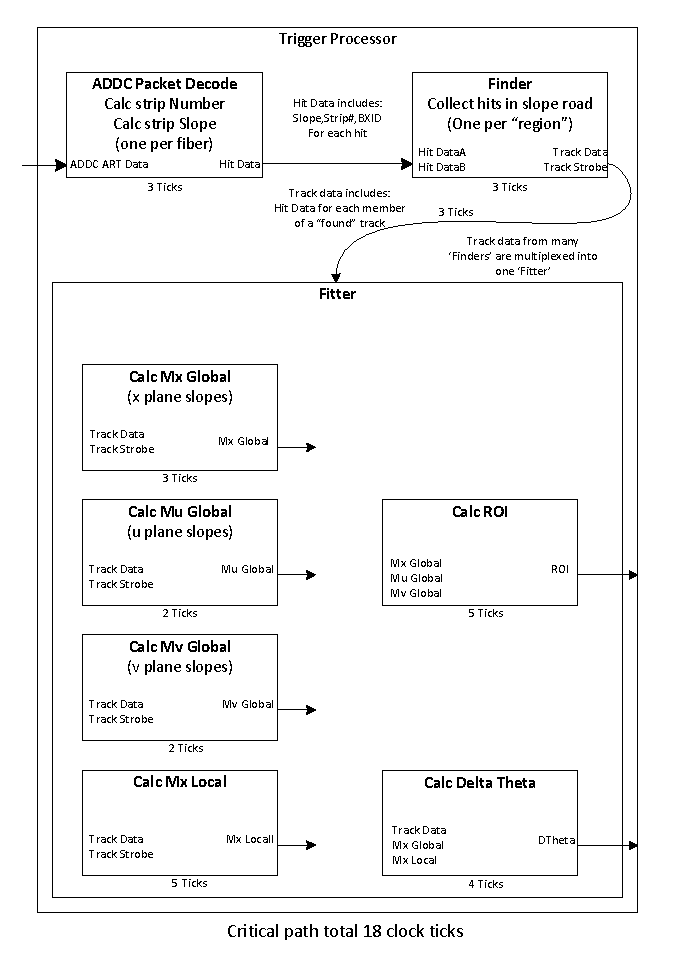
\includegraphics[width=0.7\textwidth]{algorithms-harvard/hdlBDv2.pdf}
	\caption{\label{fig:harvard_latency} Latency of the Harvard algorithm in clock ticks in each major step of the algorithm. }
	\end{center}
\end{figure} 
The last look-up table should only increase this latency by 1\,clock tick, that is to 59\,ns. Therefore, the latency time of the 
algorithm is slightly above two bunch crossings. 

\subsubsubsection{Misalignment Configurations and Corrections}

The performance in Section\,\ref{sec:harv-perf} is evaluated for ideal conditions and for
samples simulated with several misalignment effects. This section describes
the types of misalignment effects considered, how they are simulated and the
implementation of misalignment corrections in the FPGA algorithm. All misalignments
considered refer to misalignments of one multiplet with respect to the other in
the same sector. Misalignments affecting the full sector are not addressed, because they
only affect the $\theta$ and $\phi$ determination, which requires less precision. However, similar correction
techniques as those explored here can be applied to full sector position inaccuracies.

The following misalignment configurations are considered:
\begin{enumerate}\itemsep-4pt
\item $r$, displacements orthogonal to the beam axis---one or part of a multiplet shifted up or down with respect to the other,
\item $\phi$, rotations along an axis perpendicular to the wedge of one multiplet with respect to the other, with the axis
going through the center of the lower edge of the chamber,
\item $\theta_{\rm tilt}$, one plane tilted towards the IP with respect to the other,
\item $z$, one multiplet displaced along the beam axis.
\end{enumerate}
Figure\,\ref{fig:harvard_misal_illustration} illustrates each of these cases. Figures\,\ref{fig:harvard_misal_illustration}\,(a)
and~(b) correspond to two cases of the first misalignment type considered above.
\begin{figure}[htbp]
	\begin{center}
	\subfloat[a][Shift in $r$]{
		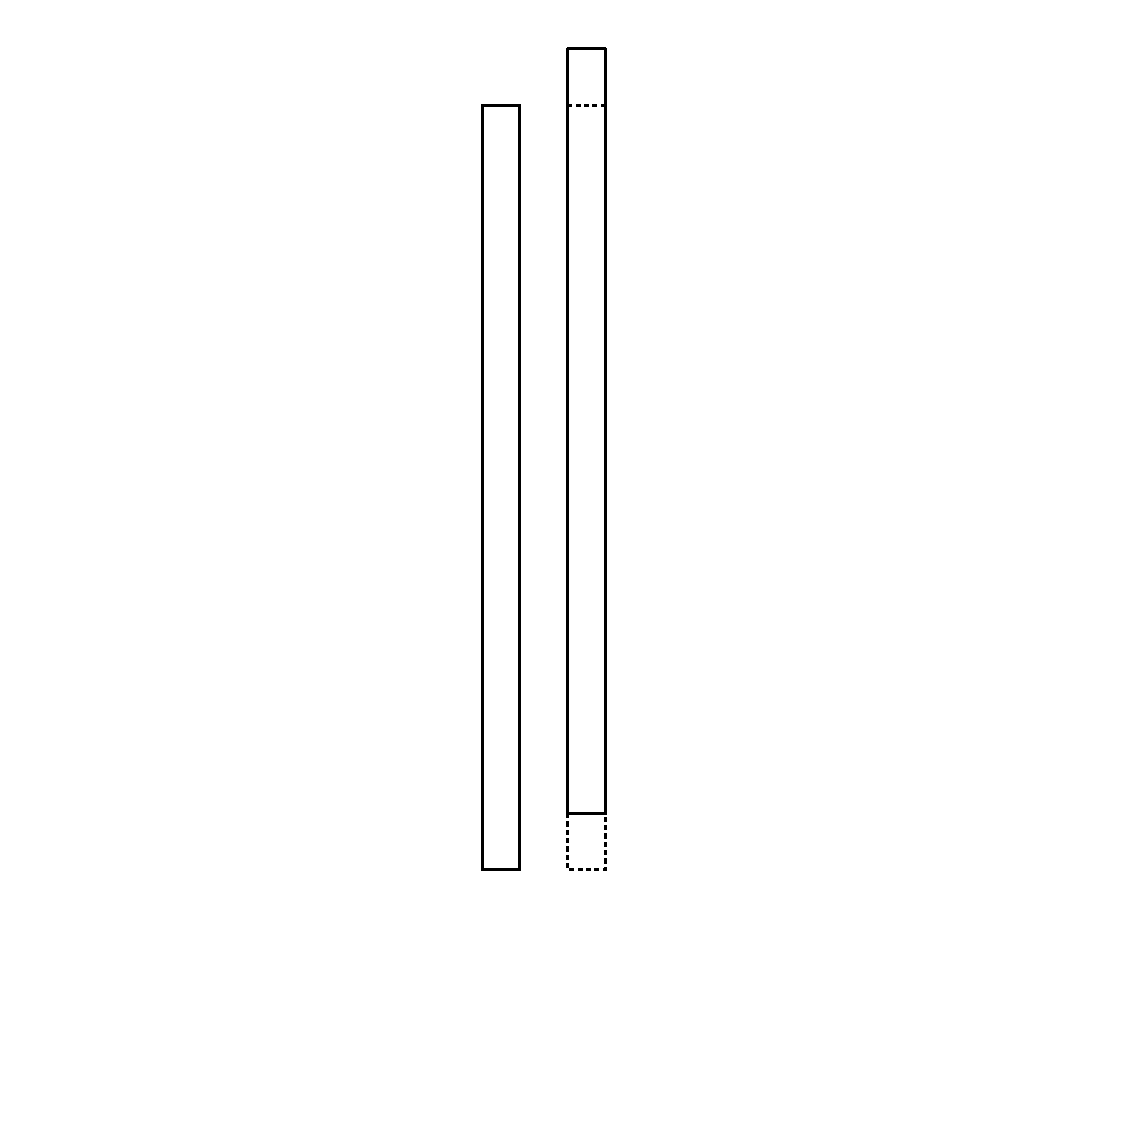
\includegraphics[trim=3.0cm 1.6cm 2.0cm 0.8cm, clip=true, width=0.19\textwidth]{algorithms-harvard/misal4.pdf}
	}
	\subfloat[b][Top half shift in $r$]{
		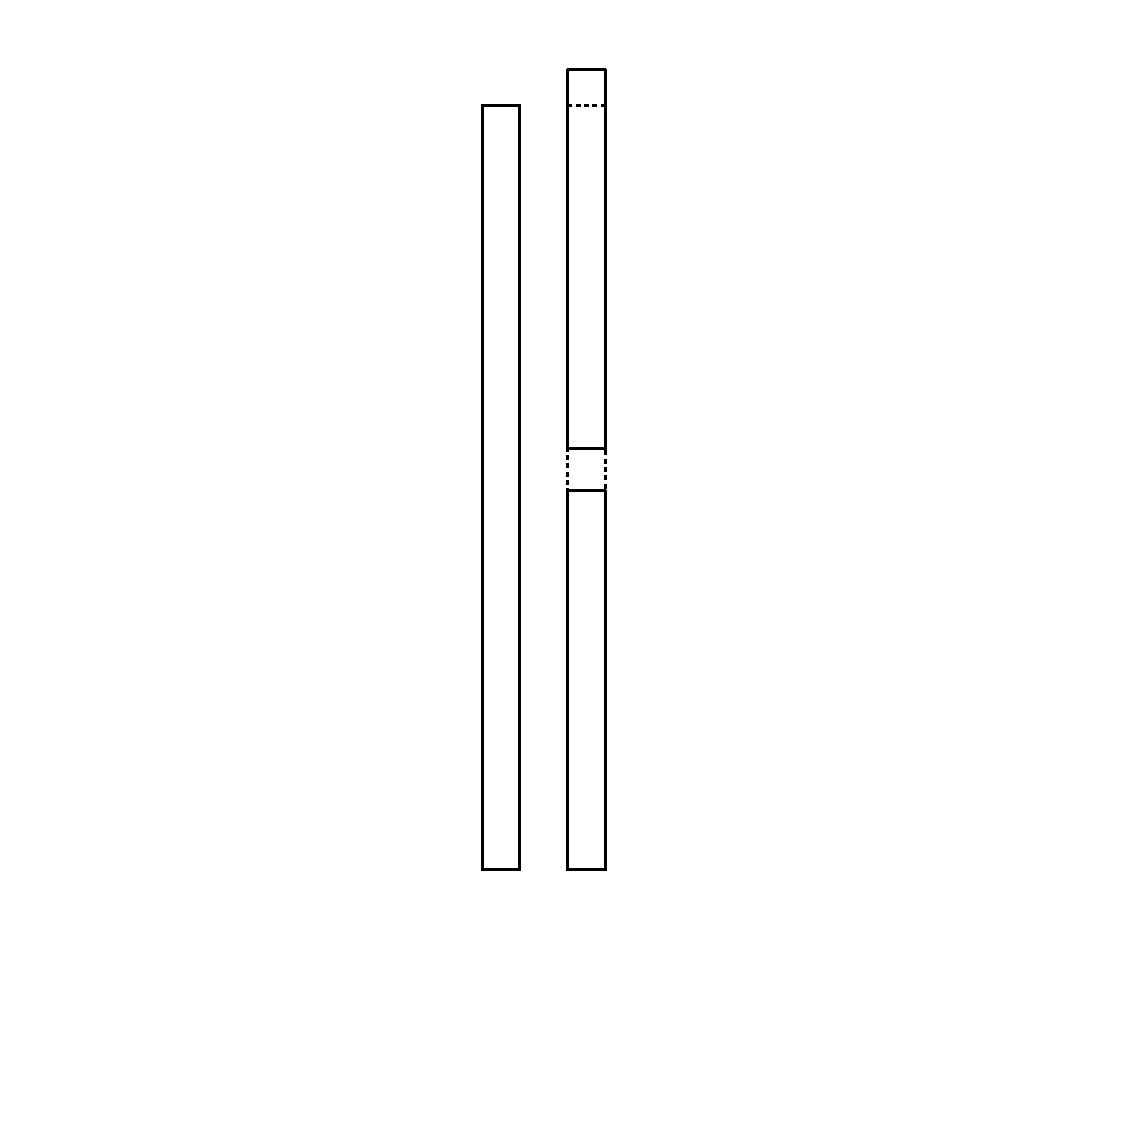
\includegraphics[trim=3.0cm 1.6cm 2.0cm 0.8cm, clip=true, width=0.19\textwidth]{algorithms-harvard/misal5.pdf}
	}
	\subfloat[c][$\phi$ rotation]{
		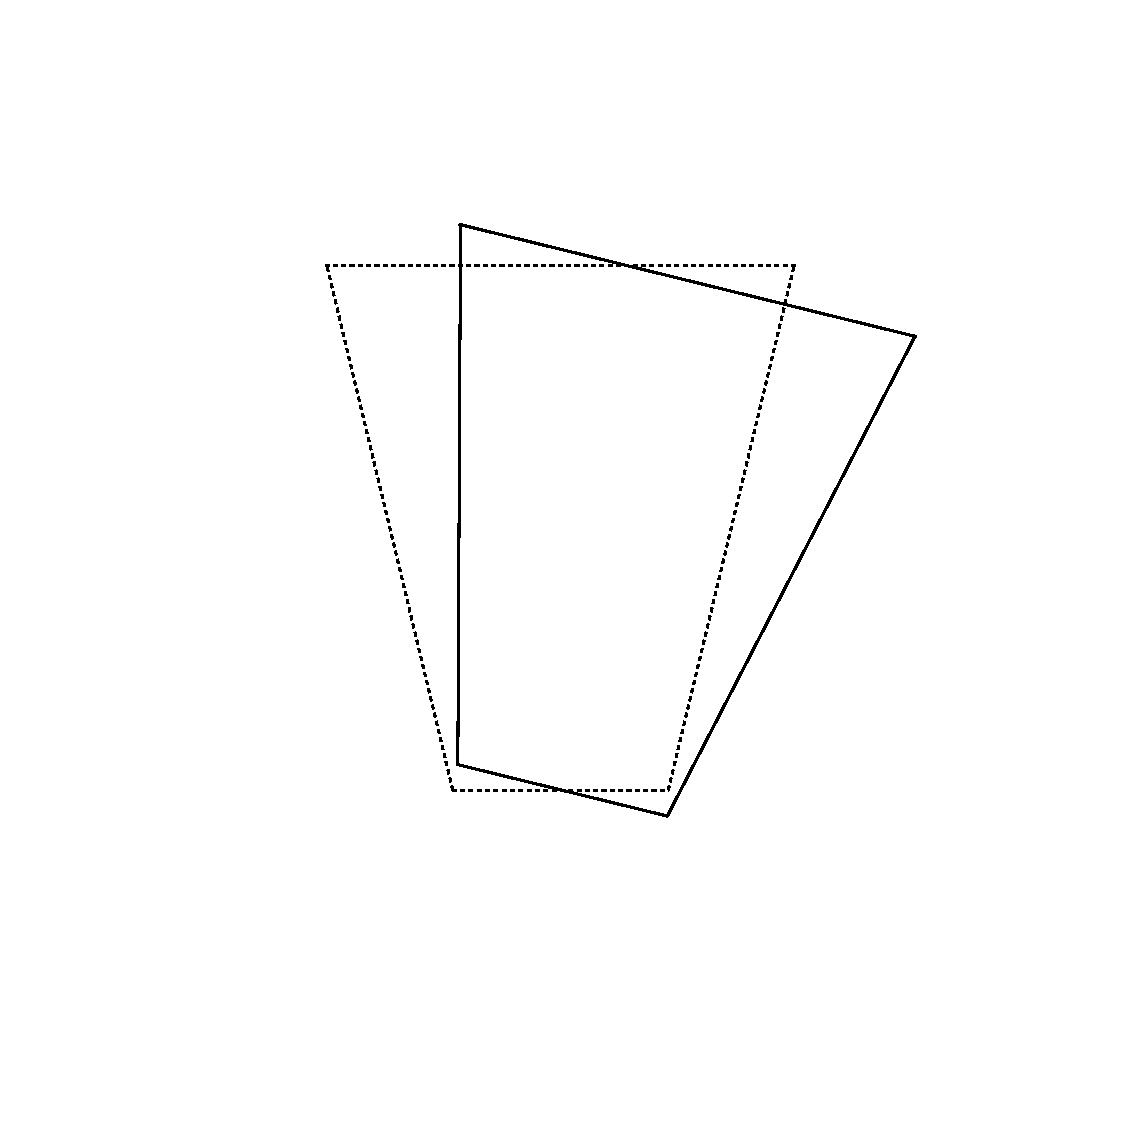
\includegraphics[trim=3.0cm 1.6cm 2.0cm 0.8cm, clip=true, width=0.19\textwidth]{algorithms-harvard/misal2.pdf}
	}
	\subfloat[d][$\theta_{\rm tilt}$]{
		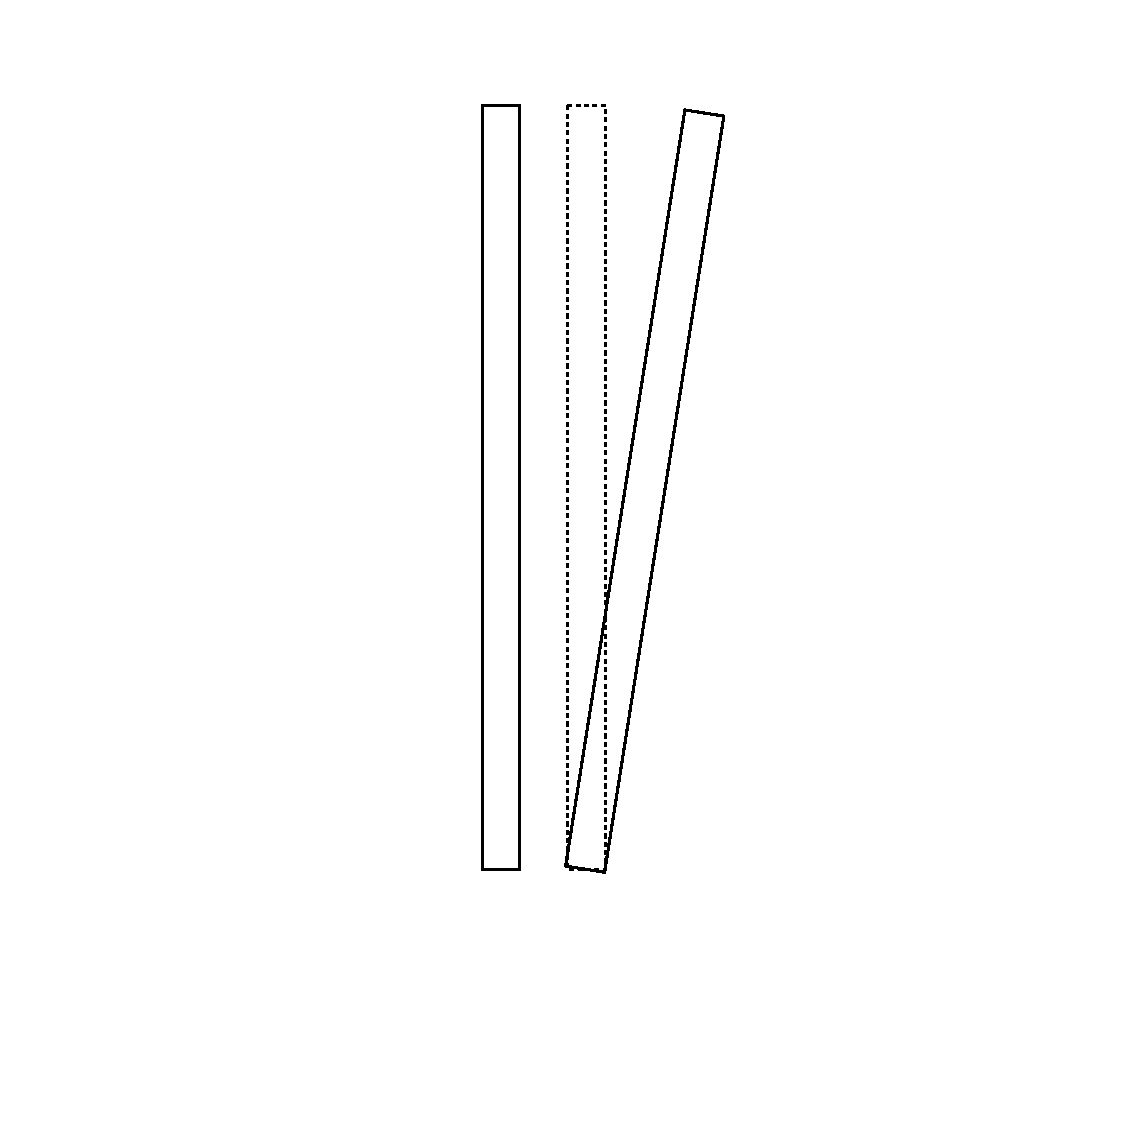
\includegraphics[trim=3.0cm 1.6cm 2.0cm 0.8cm, clip=true, width=0.19\textwidth]{algorithms-harvard/misal3.pdf}
	}
	\subfloat[e][Shift in $z$]{
		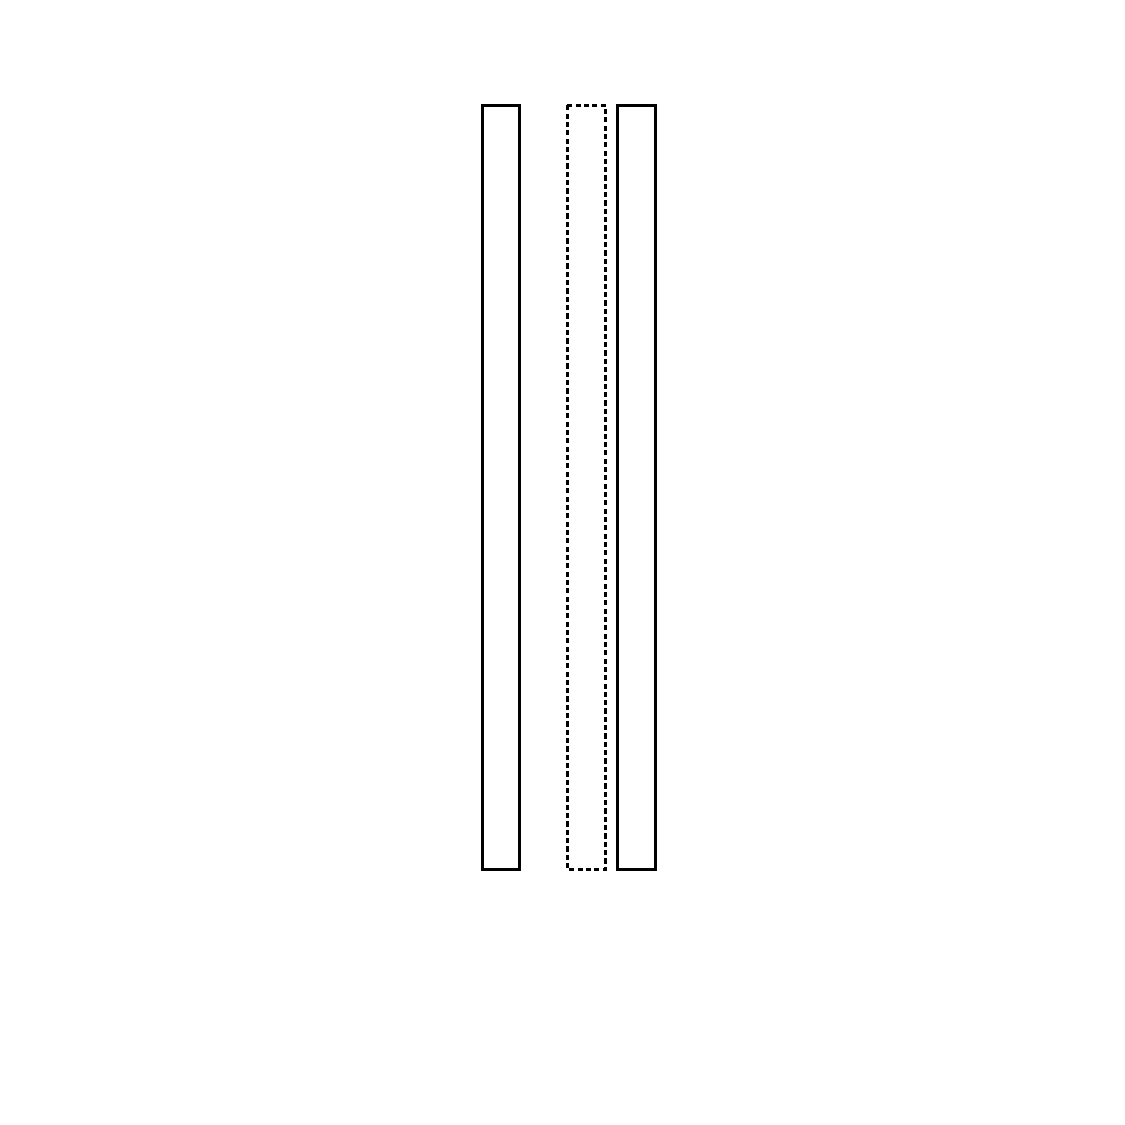
\includegraphics[trim=3.0cm 1.6cm 2.0cm 0.8cm, clip=true, width=0.19\textwidth]{algorithms-harvard/misal1.pdf}
	}

	\caption{\label{fig:harvard_misal_illustration}
	Illustration of the position of the different multiplets in the different misalignment configurations
	considered in this section. In all cases except (c), the IP is to the left and the image shows
	the $r$-$z$ plane passing through the center of the wedge. In (c), the $r$-$\phi$ plane is shown
	as it would look from the IP.
	}
	\end{center}
\end{figure}

These misalignments are simulated through the use of true hits in the Athena simulation.
The true hit position that causes the trigger to fire is known. It is thus trivial to overlay a
misaligned geometry over the true hits and recalculate the strips that were hit. Misalignments
corresponding to up to 5\,mm shifts in the relative positions of the two wedges are considered.
For the $\phi$ rotations and the $\theta_{\rm tilt}$ this corresponds to up to $1.36$\,mrad.

The performance of the trigger algorithm is studied with and without misalignments. In addition,
corrections have been implemented for all cases illustrated in Figure\,\ref{fig:harvard_misal_illustration}
except case (c). The implementation of the corrections happens in steps\,A and~E of the algorithm, described
in Section\,\ref{sec:harvard_impl}, without any additional resource overhead.
In particular, as already detailed, $2\times 8\times 16$ constants, corresponding
to 8 planes and 16 MMFEs, store the radial offset and $z$ position of the corresponding strips. These constants
can be updated to perfectly counteract the effects of the cases illustrated above in (a), (b) and (e). Case
(d) can also be corrected with some loss of accuracy, since only 16 $z$ positions are stored along the tilted
plane. The $z$ positions stored can be optimized, but for the studies in this document the middle $z$ position
of the strips read out by each MMFE is used. The loss of accuracy from this simplified corrections is quantified
in the next section. Corrections for case (c) have not been studied yet, but the effects of such a misalignment
have been studied and are shown in the next section.

%%%%%%%%%%%%%%%%%%%%%%%%%%%%%%%%%%%
\subsubsubsection{Performance}
\label{sec:harv-perf}

The performance of the algorithm is studied using single muon events generated with Athena
full simulation. A geometry with two equal quadruplets each with two horizontal strips and two
different-tilt stereo strips (xxuv) was used. Most of the studies used here use a geometry
in which the quadruplets are placed with horizontal strips placed closer to the IP
(xxuv xxuv).

The samples were generated using muons generated at the IP. However, additional
samples with typical parameters of the ATLAS beamspot during Run\,1
using for the origin of the muons Gaussian distributions of mean $(x,y,z)=(0.05,0.06,-1)$\,mm
and $(\sigma_x,\sigma_y,\sigma_z)=(0.01,0.01,70)$\,mm have also been checked. The
results with the samples with realistic beamspot (not shown here) result in a degradation of
the $\theta$ resolution of about a factor of two, but no noticeable effects on the $\Delta\theta$
or $\phi$ resolutions or the trigger efficiency.
Two samples using
muons with energies of 200 and 1000\,\GeV have been studied. Each sample has 20000 events
with muons pointing to one large sector of the NSW.
Of the digitized hits found in the simulation, the first
registered signal per channel was chosen for trigger construction.
A function mimicking a VMM chip's 100\,ns deadtime and coverage of
64 strips was also applied to the data.  This function serves to guarantee a
maximum of one hit, true or background, is registered for each 64 grouping of strips for each event.

Three set of studies complement the performance studies in ideal conditions:
\begin{itemize}\itemsep-4pt
\item a study of the effects of incoherent background,
\item a study of the impact of misalignments and the corrections designed to mitigate them,
\item a study of the performance with quadruplets with mirror-image placement (xxuv uvxx), proposed recently
to increase the lever-arm for fitting the bending coordinate using horizontal (x) strips.
\end{itemize}

The following variables are used to parameterize performance. Fit efficiency is defined as the efficiency
for a track to trigger the detector given that a minimum number of trigger hits before including background exist.
In particular, n-horizontal/n-stereo refers to events for which there were at least n hits in the horizontal strips and
the same amount in the stereo strips before addition of background hits. Distributions are calculated with respect
to truth definitions. In particular, the distributions of $\theta^{\rm{fit}}-\theta^{\rm{true}}$,
$\phi^{\rm{fit}}-\phi^{\rm{true}}$, and $\Delta\theta^{\rm{fit}}-\Delta\theta^{\rm{true}}$, for which true coordinates and direction
are defined at the entrance of the NSW, are studied. The distributions are fit using Gaussian fits with a one-step recursive
fit. The raw results are first fitted to a gaussian. The quoted resolutions are obtained through a fit in the range
$[\mu_1-3\sigma_1,\mu_1+3\sigma_1]$, where $\mu_1$ and $\sigma_1$ are the mean and standard deviation of the first fit. Tails
are defined as the fraction of events outside the range $[\mu_1-3\sigma_1,\mu_1+3\sigma_1]$.

Sample distributions, integrated over all $\eta$, are shown for the $\phi$, $\theta$ and $\Delta\theta$ reconstruction
in Figures\,\ref{fig:phi_harvard}, \ref{fig:theta_harvard} and \ref{fig:dtheta_harvard}.
\begin{figure}[htbp]
	\centering
%	\subfloat[a][]{
%		\includegraphics[width=0.33\textwidth]{algorithms-harvard/50GeVphi_etaall.pdf}
%	}
	\subfloat[a][]{
		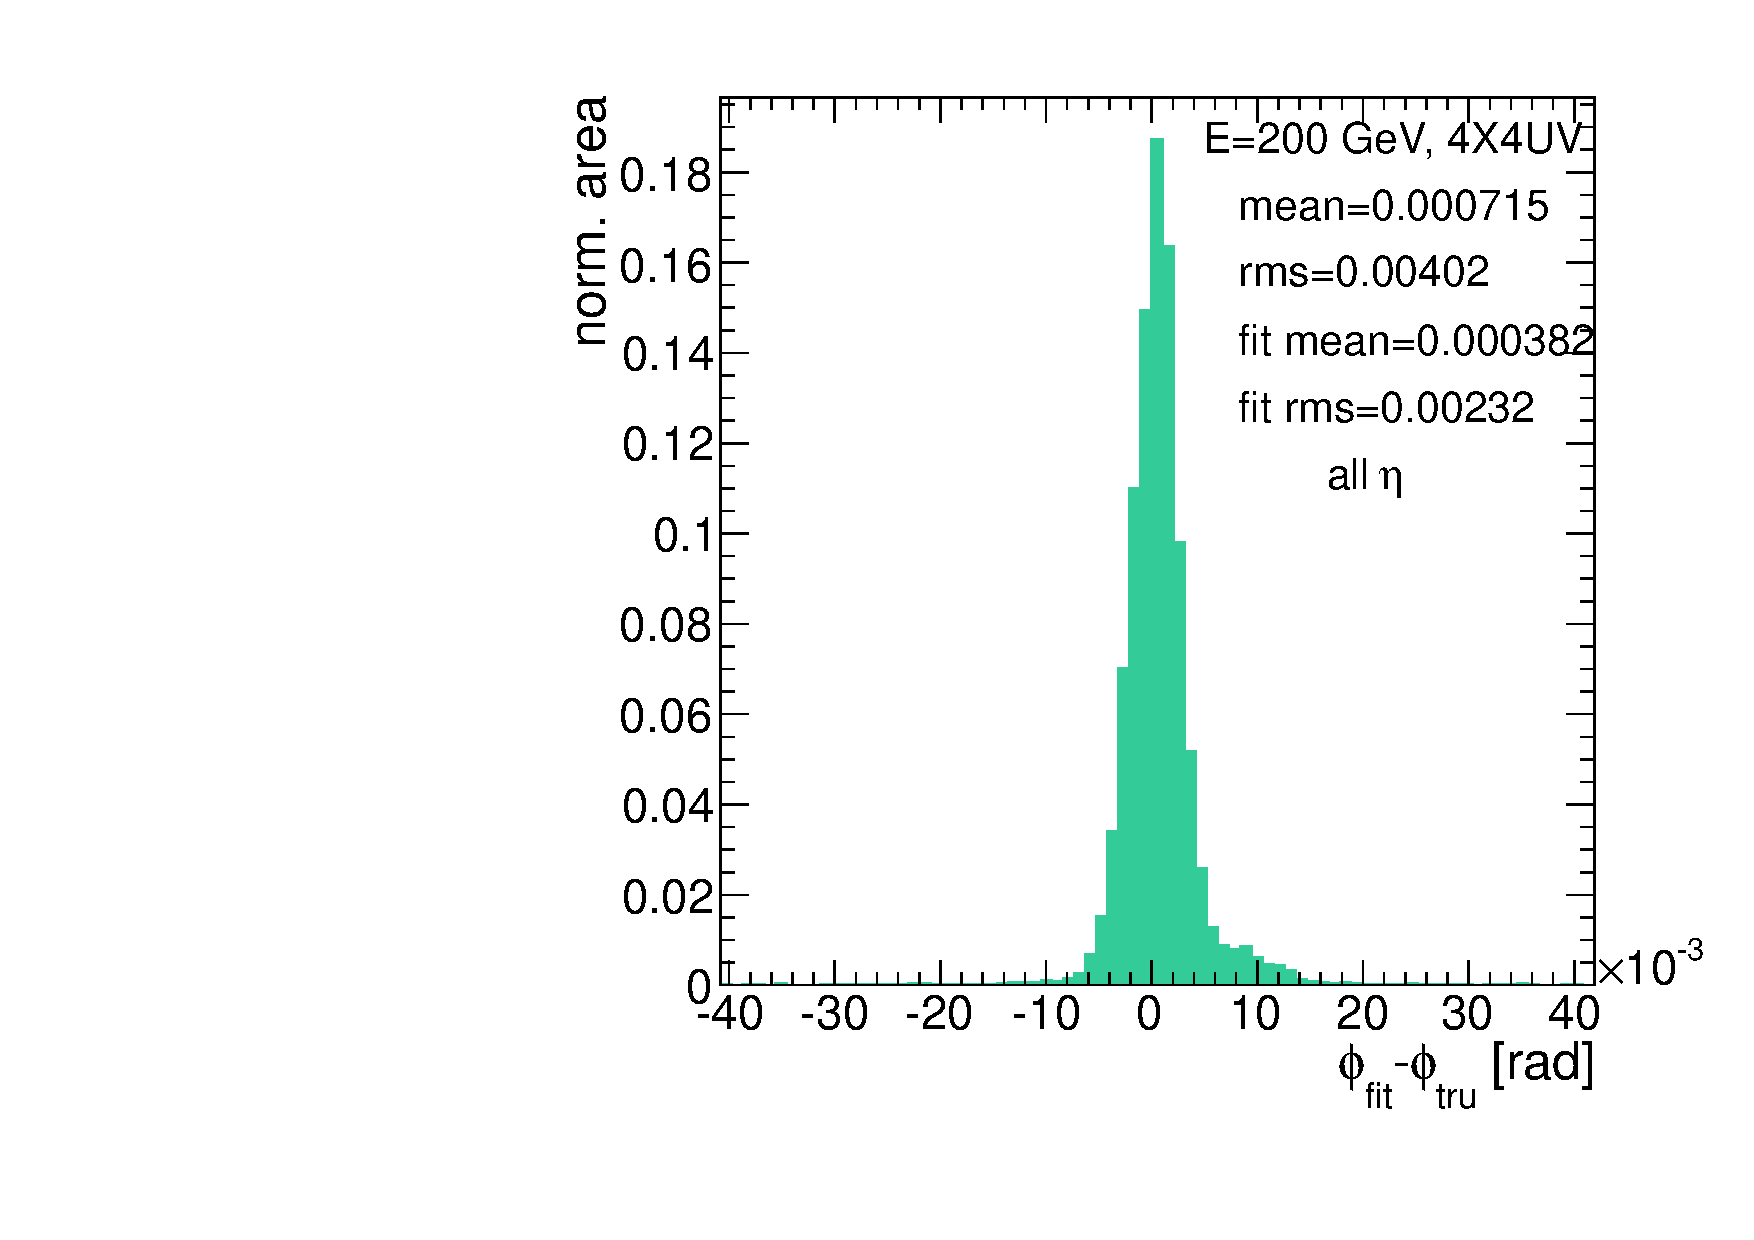
\includegraphics[width=0.4\textwidth]{algorithms-harvard/200GeVphi_etaall.pdf}
	}
	\subfloat[b][]{
		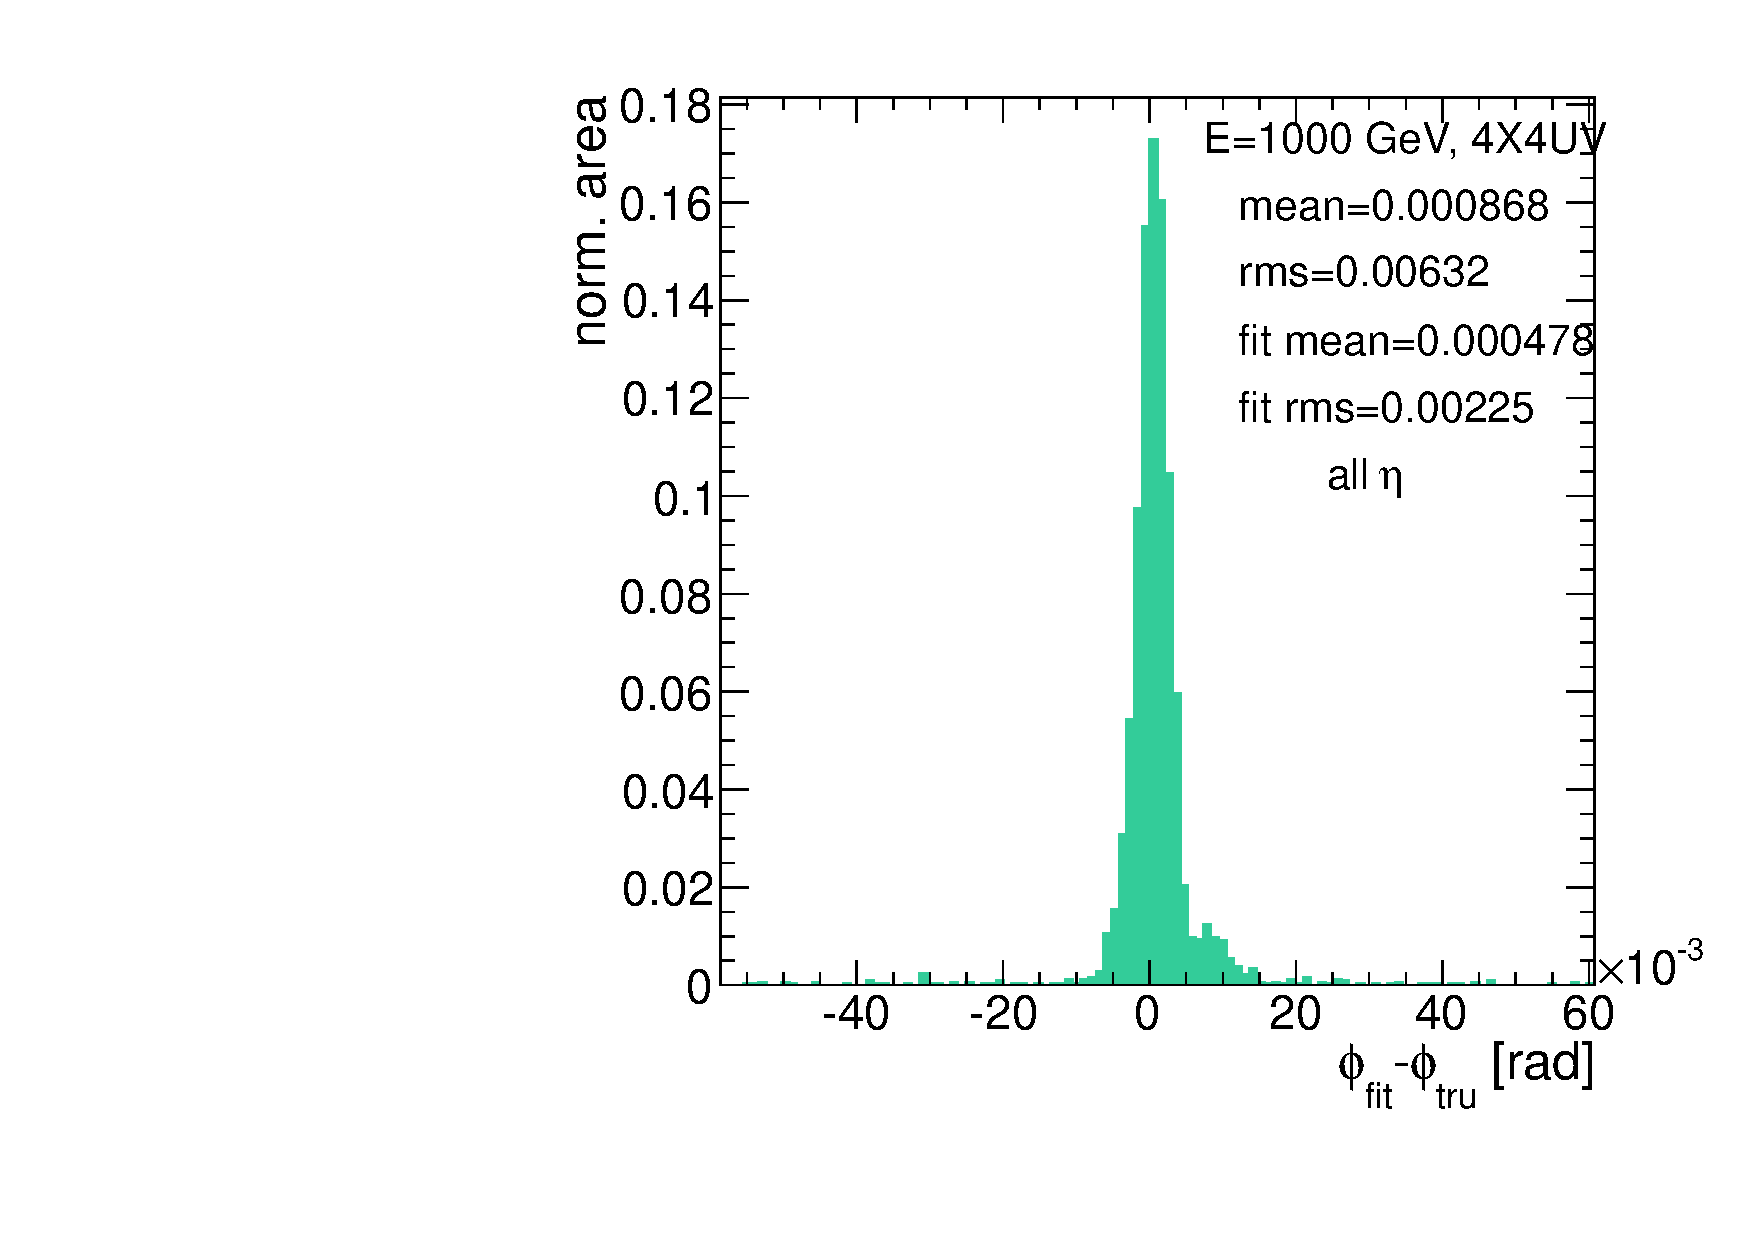
\includegraphics[width=0.4\textwidth]{algorithms-harvard/1000GeVphi_etaall.pdf}
	}\\
	\caption{\label{fig:phi_harvard}
Distribution of reconstructed $\phi$ minus true $\phi$ value of the track at the entrance of the NSW
for muons of $E=200\GeV$ (a) and $E=1\TeV$ (b). The xxuv xxuv configuration without background
is used.
	}
\end{figure}

\begin{figure}[htbp]
	\centering
%	\subfloat[a][]{
%		\includegraphics[width=0.33\textwidth]{algorithms-harvard/50GeVtheta_etaall.pdf}
%	}
	\subfloat[a][]{
		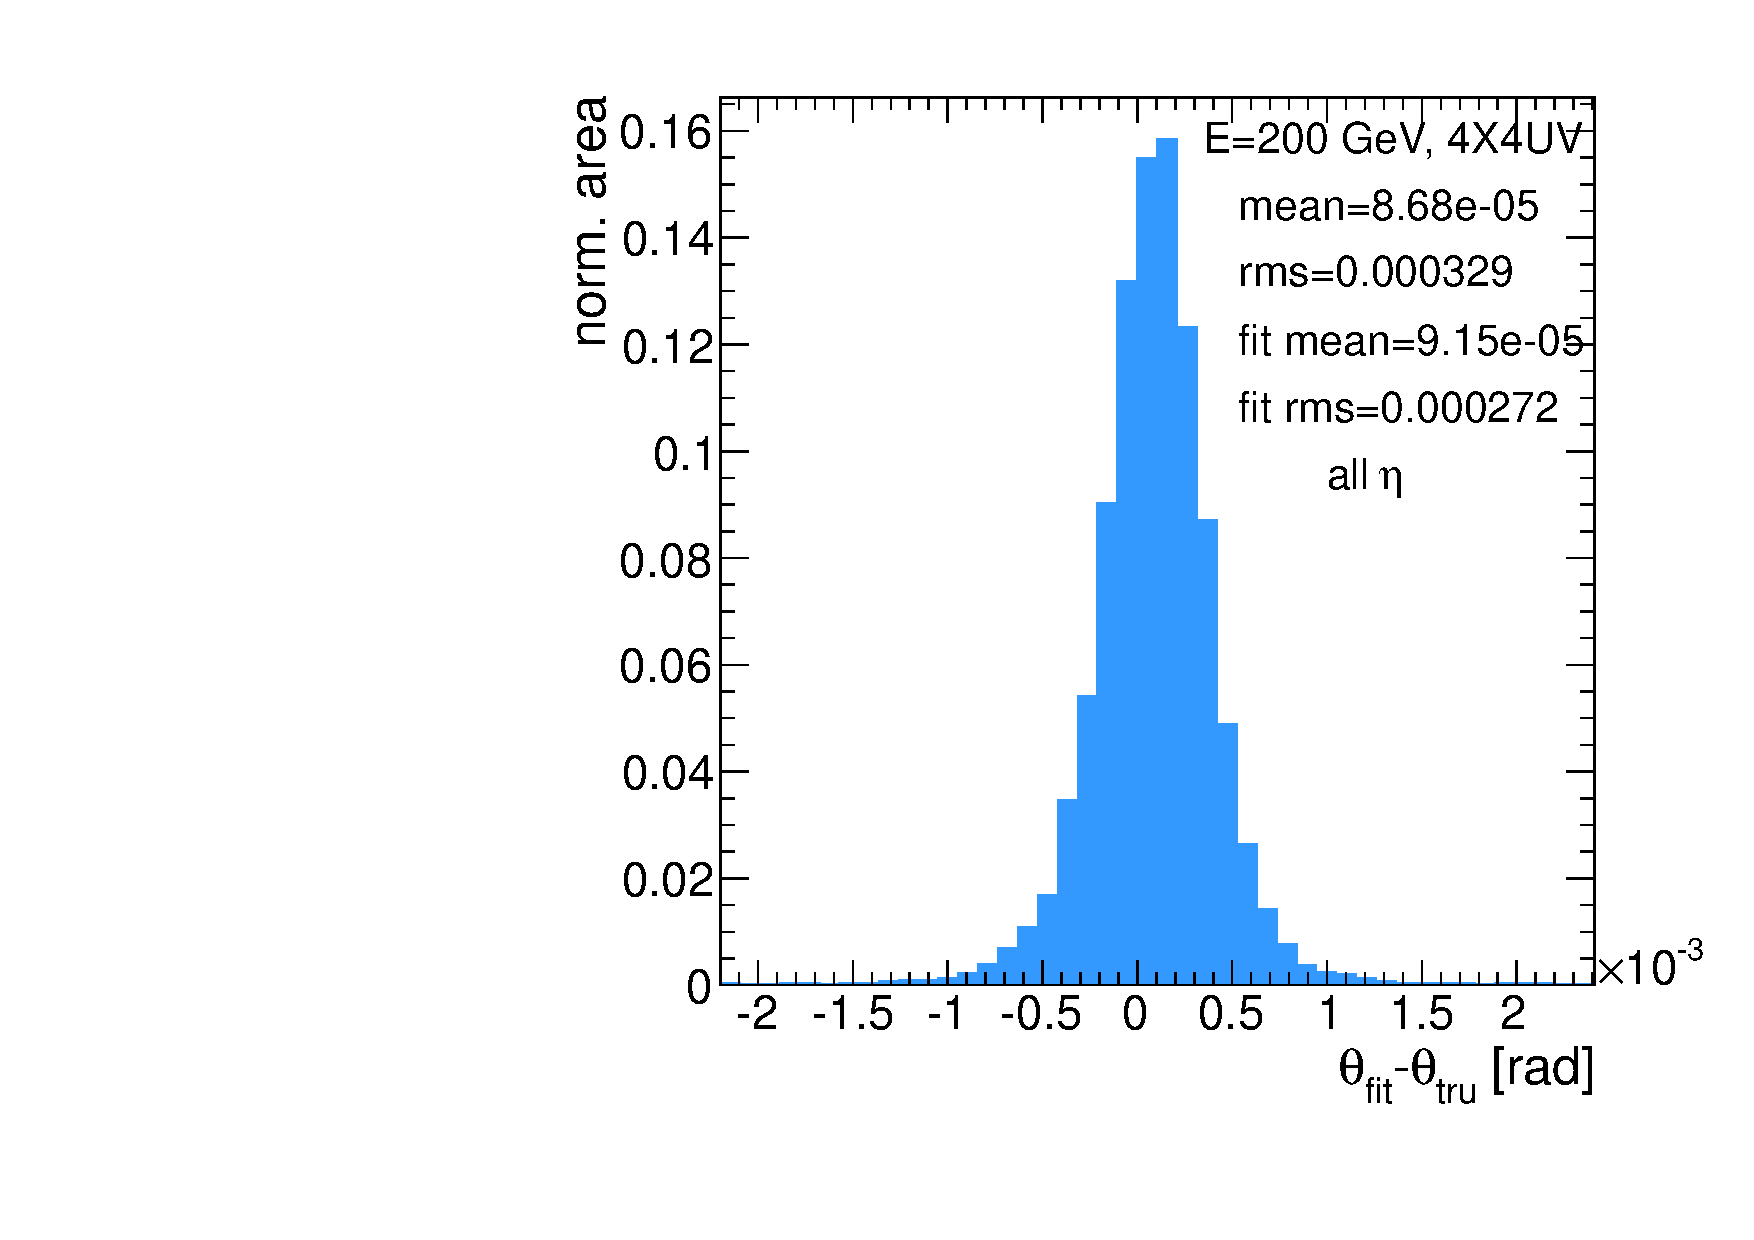
\includegraphics[width=0.45\textwidth]{algorithms-harvard/200GeVtheta_etaall.pdf}
	}
	\subfloat[b][]{
		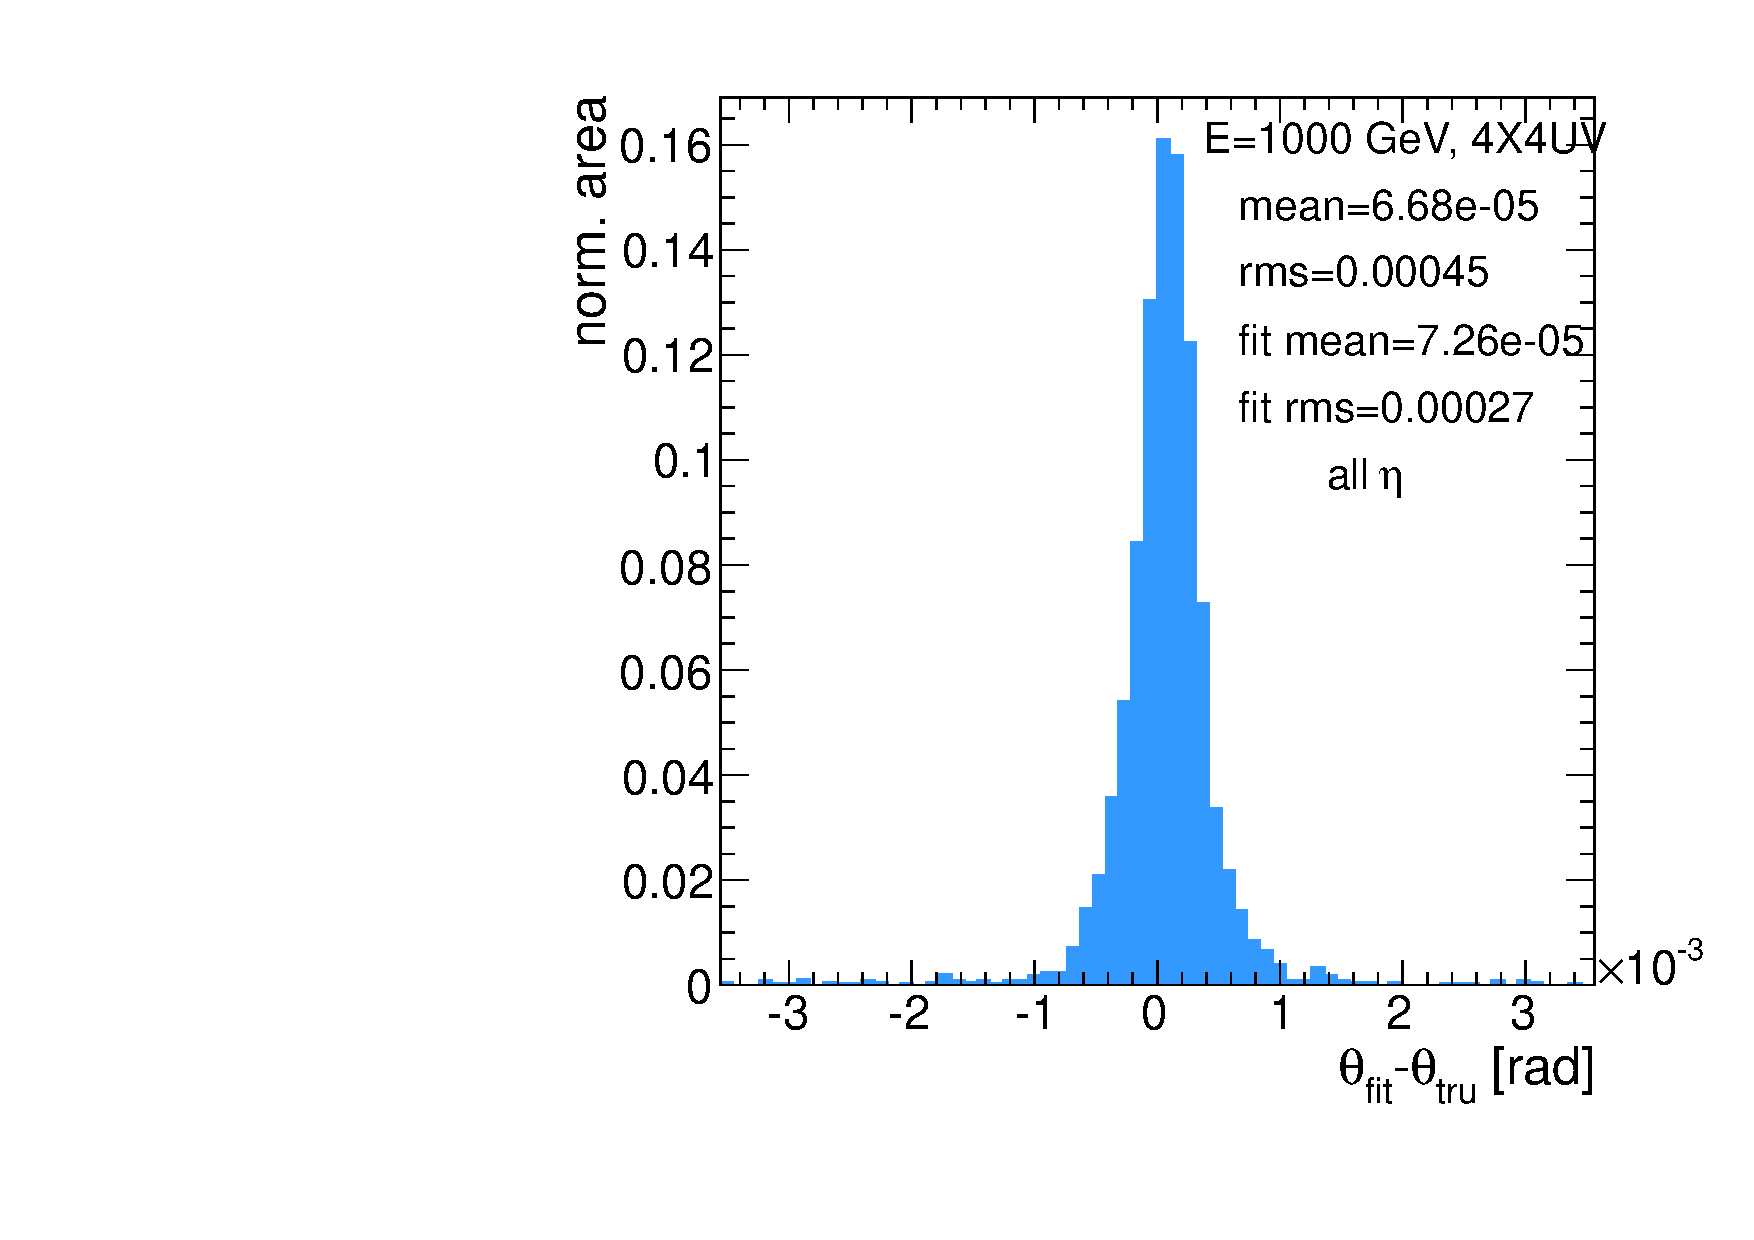
\includegraphics[width=0.45\textwidth]{algorithms-harvard/1000GeVtheta_etaall.pdf}
	}\\
	\caption{\label{fig:theta_harvard}
Distribution of reconstructed global $\theta$ minus true global $\theta$ value of the track at the entrance of the NSW
for muons of $E=200\GeV$ (a) and $E=1\TeV$ (b). The xxuv xxuv configuration without background
is used.
	}
\end{figure}

\begin{figure}[htbp]
	\centering
%	\subfloat[a][]{
%		\includegraphics[width=0.33\textwidth]{algorithms-harvard/50GeVdtheta_etaall.pdf}
%	}
	\subfloat[a][]{
		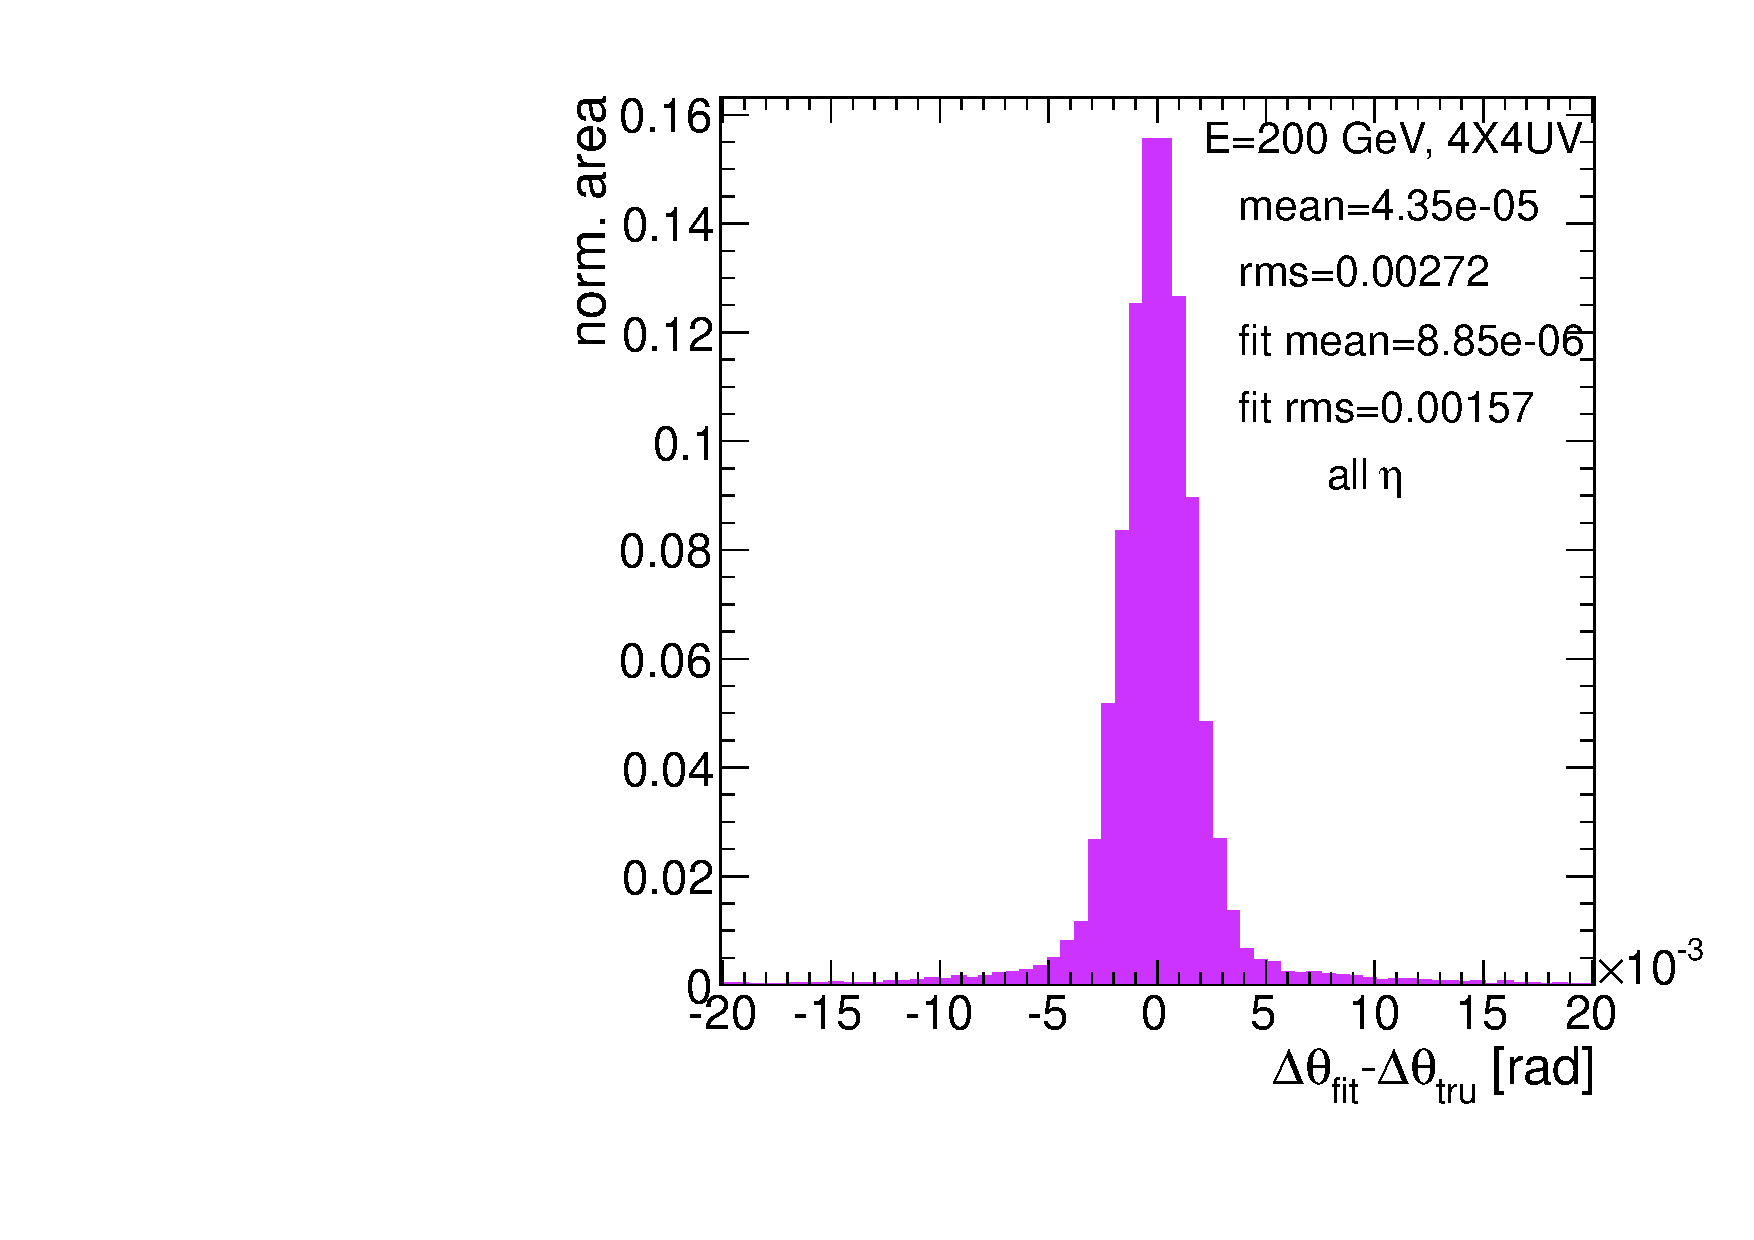
\includegraphics[width=0.45\textwidth]{algorithms-harvard/200GeVdtheta_etaall.pdf}
	}
	\subfloat[b][]{
		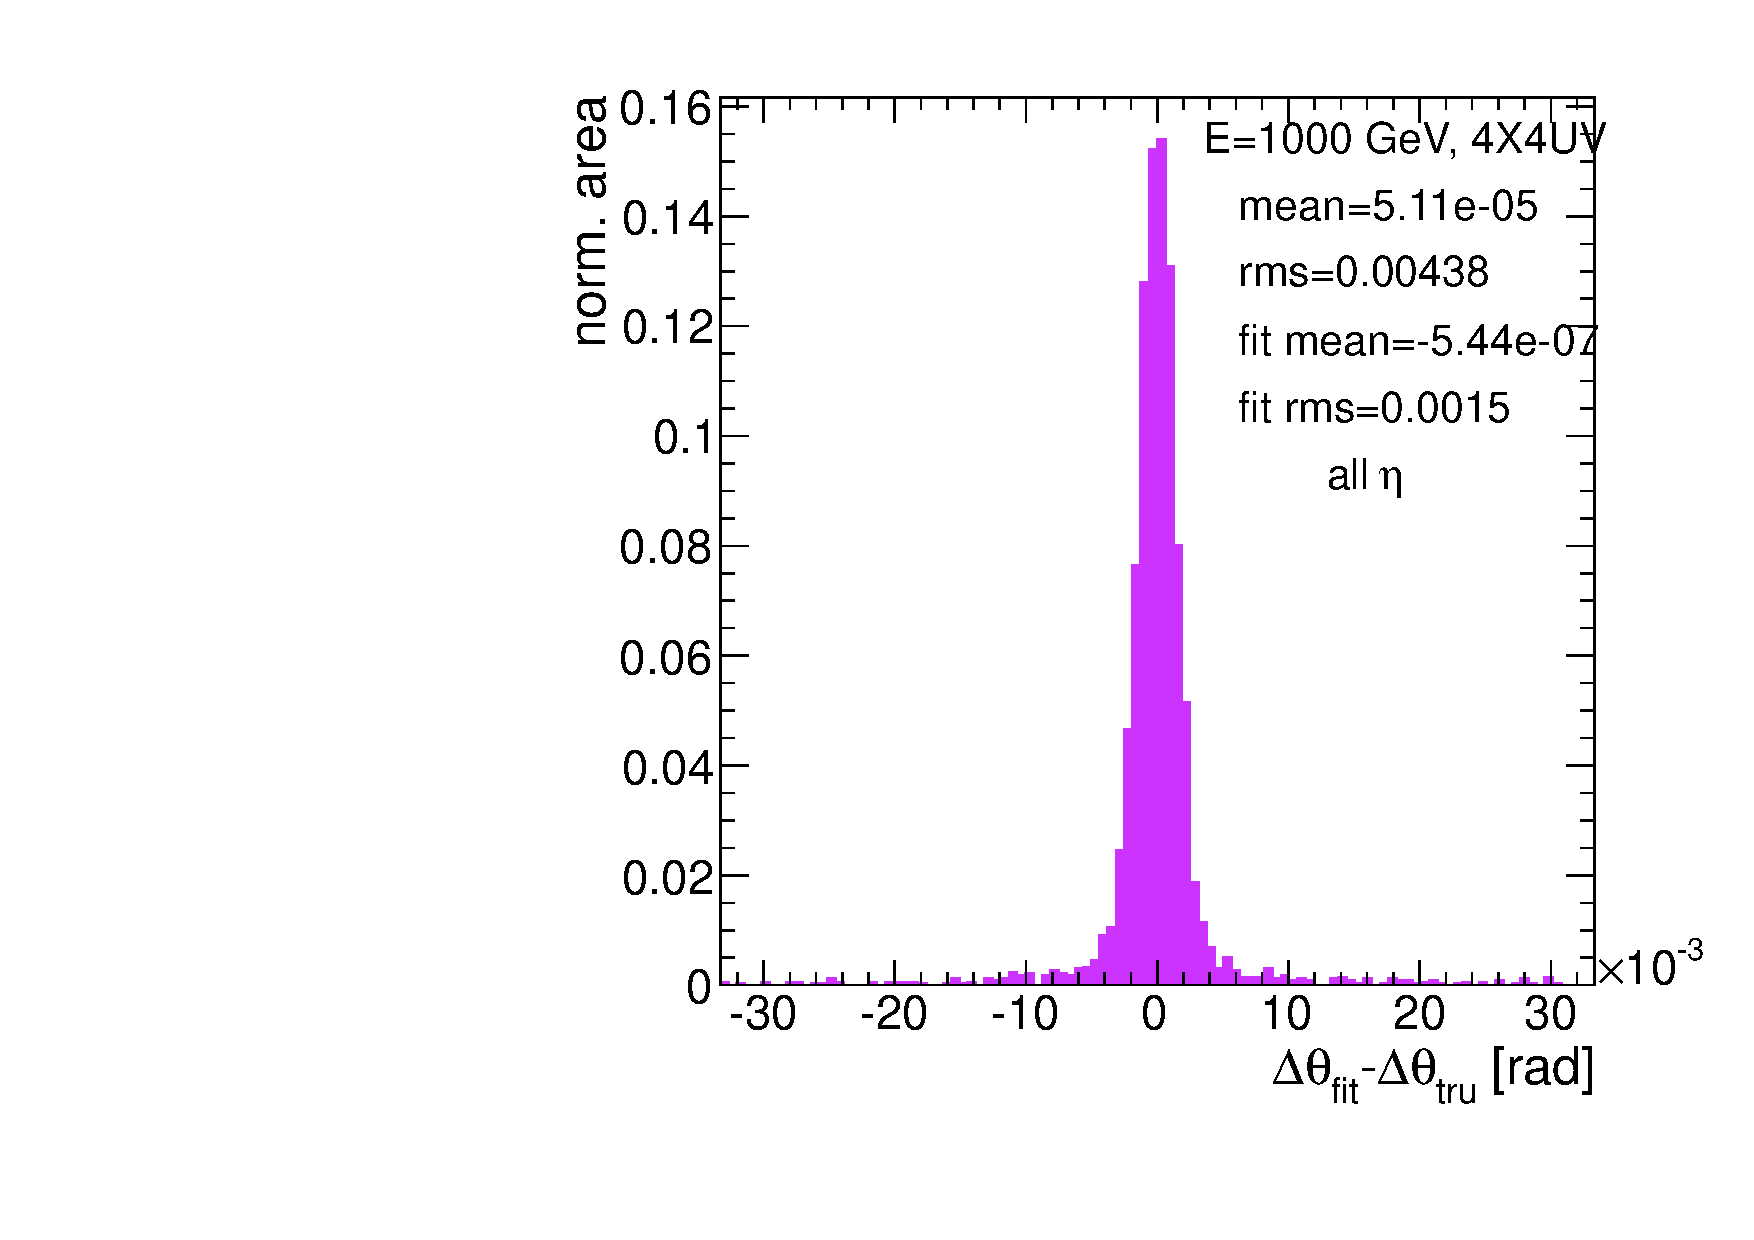
\includegraphics[width=0.45\textwidth]{algorithms-harvard/1000GeVdtheta_etaall.pdf}
	}\\
	\caption{\label{fig:dtheta_harvard}
Distribution of reconstructed $\Delta\theta$ minus true $\Delta\theta$ value of the track at the entrance of the NSW
for muons of $E=200\GeV$ (a) and $E=1\TeV$ (b). The xxuv xxuv configuration without background
is used.
	}
\end{figure}

The distributions do not change significantly with energy, except for an increase in the tails for the highest
energy studied. This is caused by an increase in events with large number of secondary particles,
which throw off the fit when they occur.

Figure~\ref{fig:harvard_ideal_eff}~(a) shows the efficiency of the algorithm for events for which
truth hits are found for different thresholds. The $E=200\GeV$ sample and an ideal geometry
without background is used. The efficiency increases with the number of hits as expected because
of the extra redundancy added by the additional hits, which makes the fit more likely to succeed
even if some hits are not usable. The efficiency of the algorithm is very close to 100\%.
Figure~\ref{fig:harvard_ideal_eff}~(b) shows the true efficiency of each category, where the denominator
includes all muons at the entrance of the spectrometer. In this case the x-axis should be interpreted as
an inclusive axis (the 2X, 1U or 1V case refers to tracks with at least that many hits, so it includes all
events falling in the other bins). This figure thus includes the algorithmic efficiency in Figure~\ref{fig:harvard_ideal_eff}~(a)
and the detector efficiency. It also gives a quantitative answer about the fraction of tracks with a given
number of coincidence threshold requirements. Finally, Figure~\ref{fig:harvard_ideal_eff}~(c) shows the efficiency with the
same definition as was used in Figure~\ref{fig:SaclayEfficiencyForDifferentPairRequirement} for easy comparison. It should
be noted that the minimum fit requirement in Figure~\ref{fig:harvard_ideal_eff}~(c) is two horizontal strips and one stereo
strip. This is a rather loose requirement, so it should be no surprise that the efficiencies are higher than for Figure~\ref{fig:SaclayEfficiencyForDifferentPairRequirement}. However, tighter requirements can also be observed in the
figure as the x axis increases.
\begin{figure}[htbp]
	\centering
	\subfloat[a][]{
		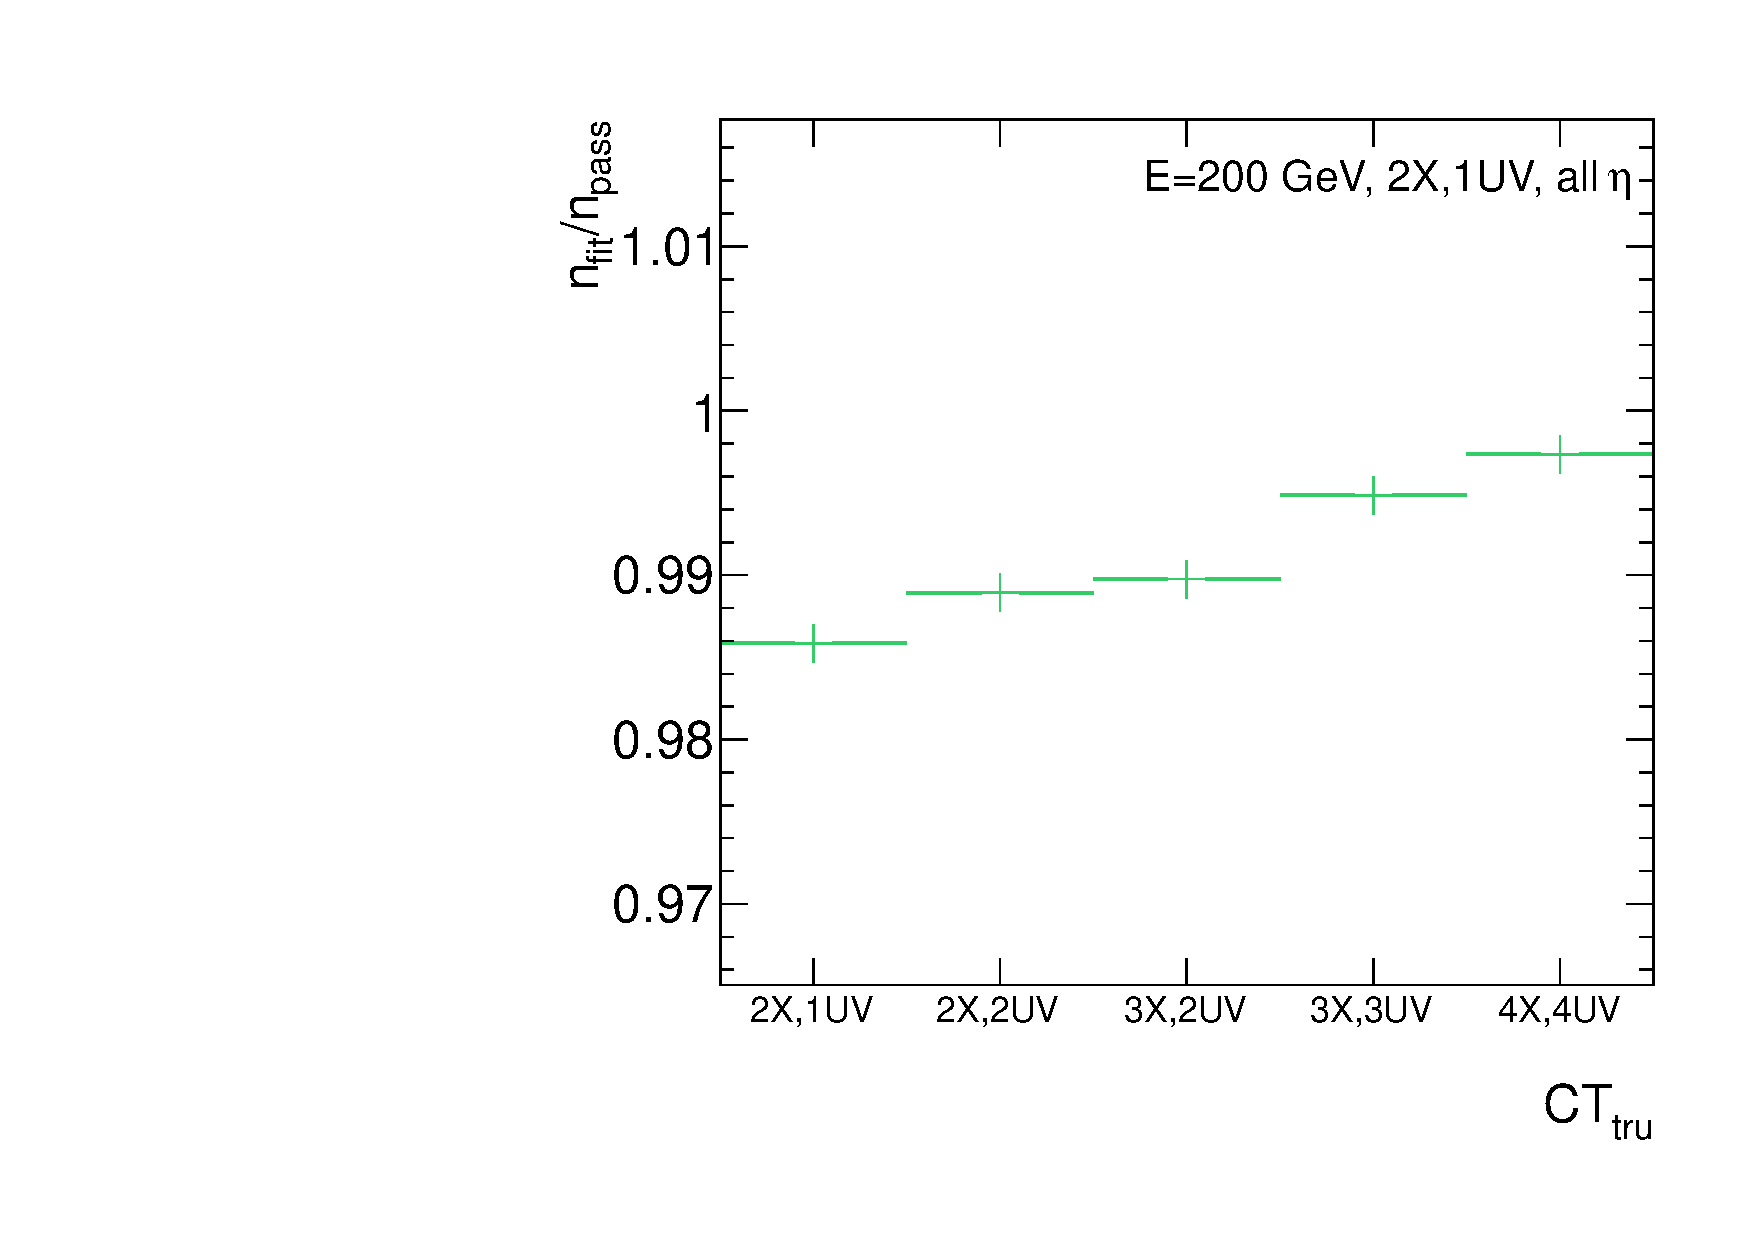
\includegraphics[width=0.33\textwidth]{algorithms-harvard/ct_var_2x_1uv_etaall_eff_note_200GeV.pdf}
	}
	\subfloat[b][]{
		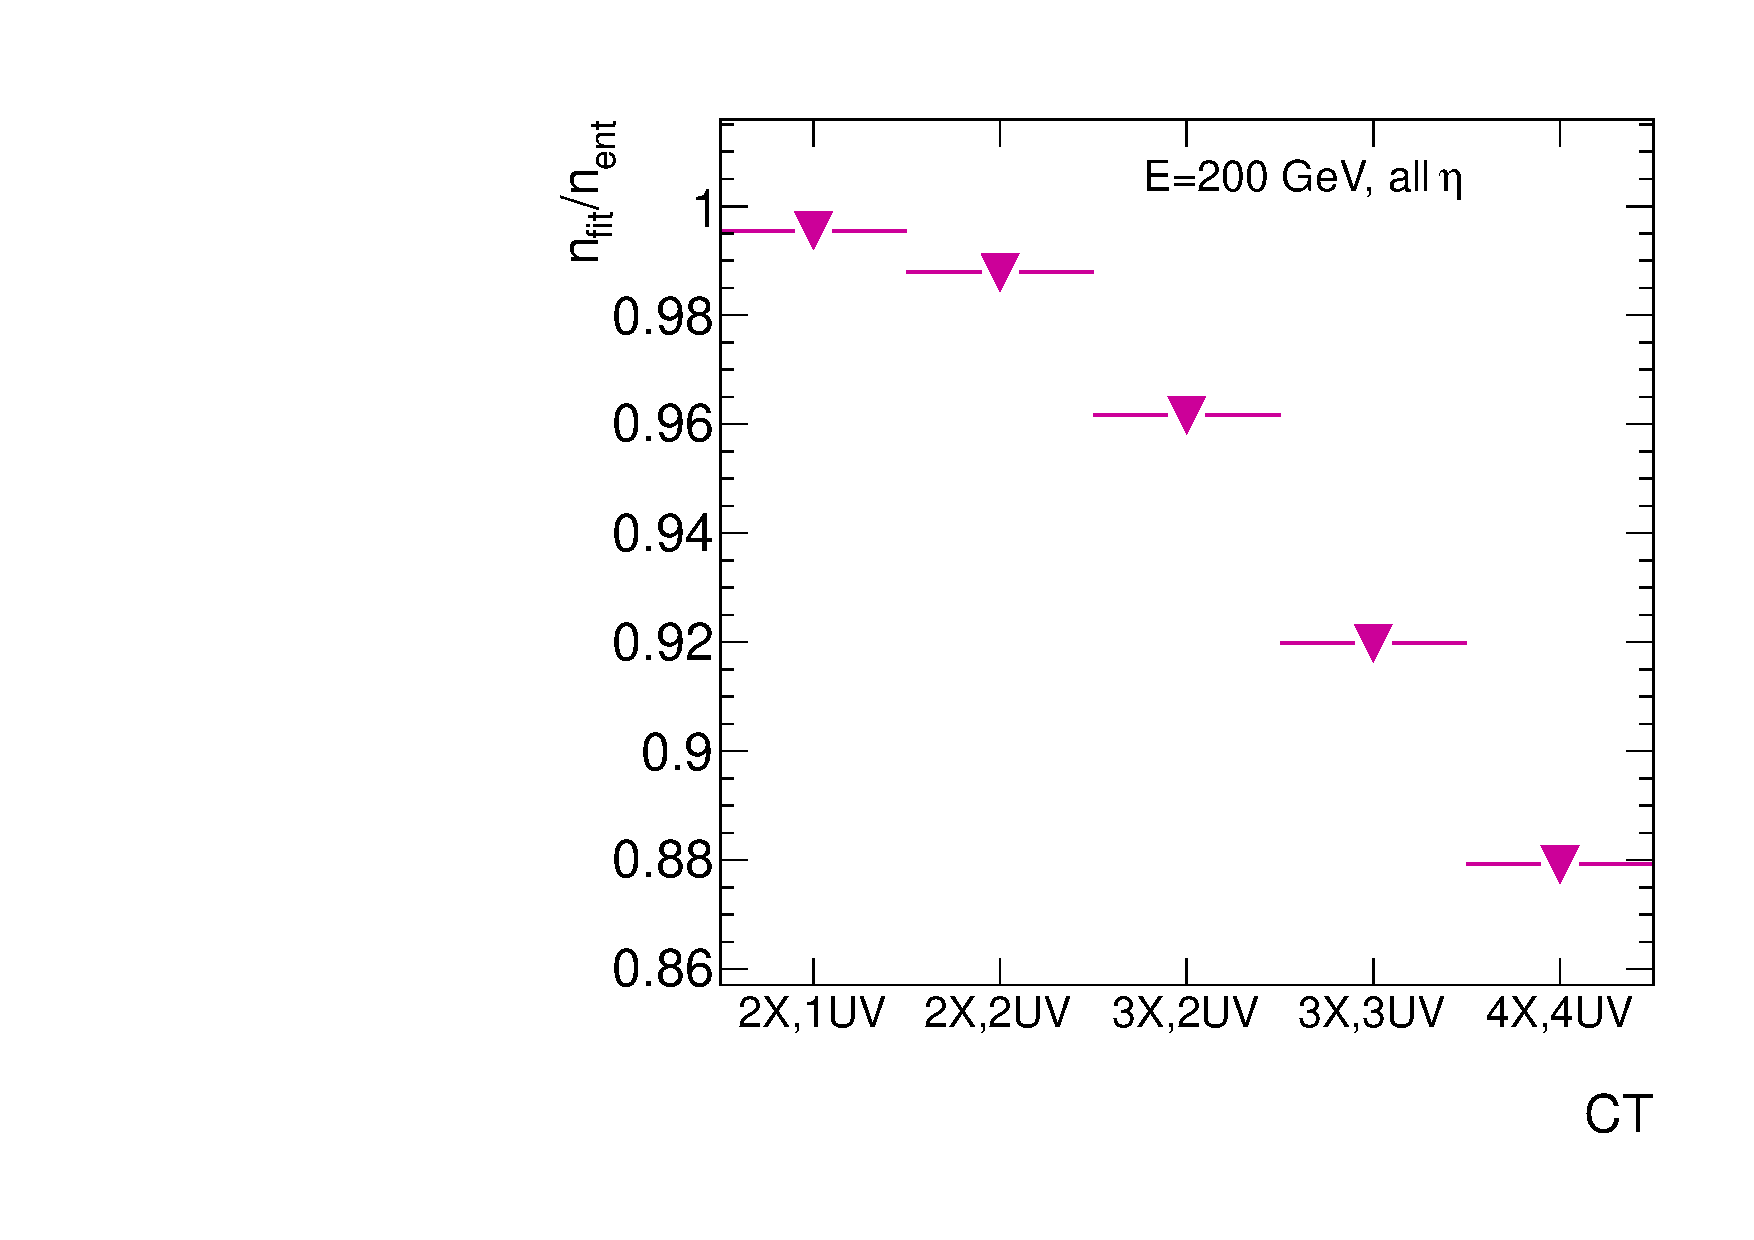
\includegraphics[width=0.33\textwidth]{algorithms-harvard/ct_var_etaall_eff_tru_200GeV.pdf}
	}
	\subfloat[c][]{
	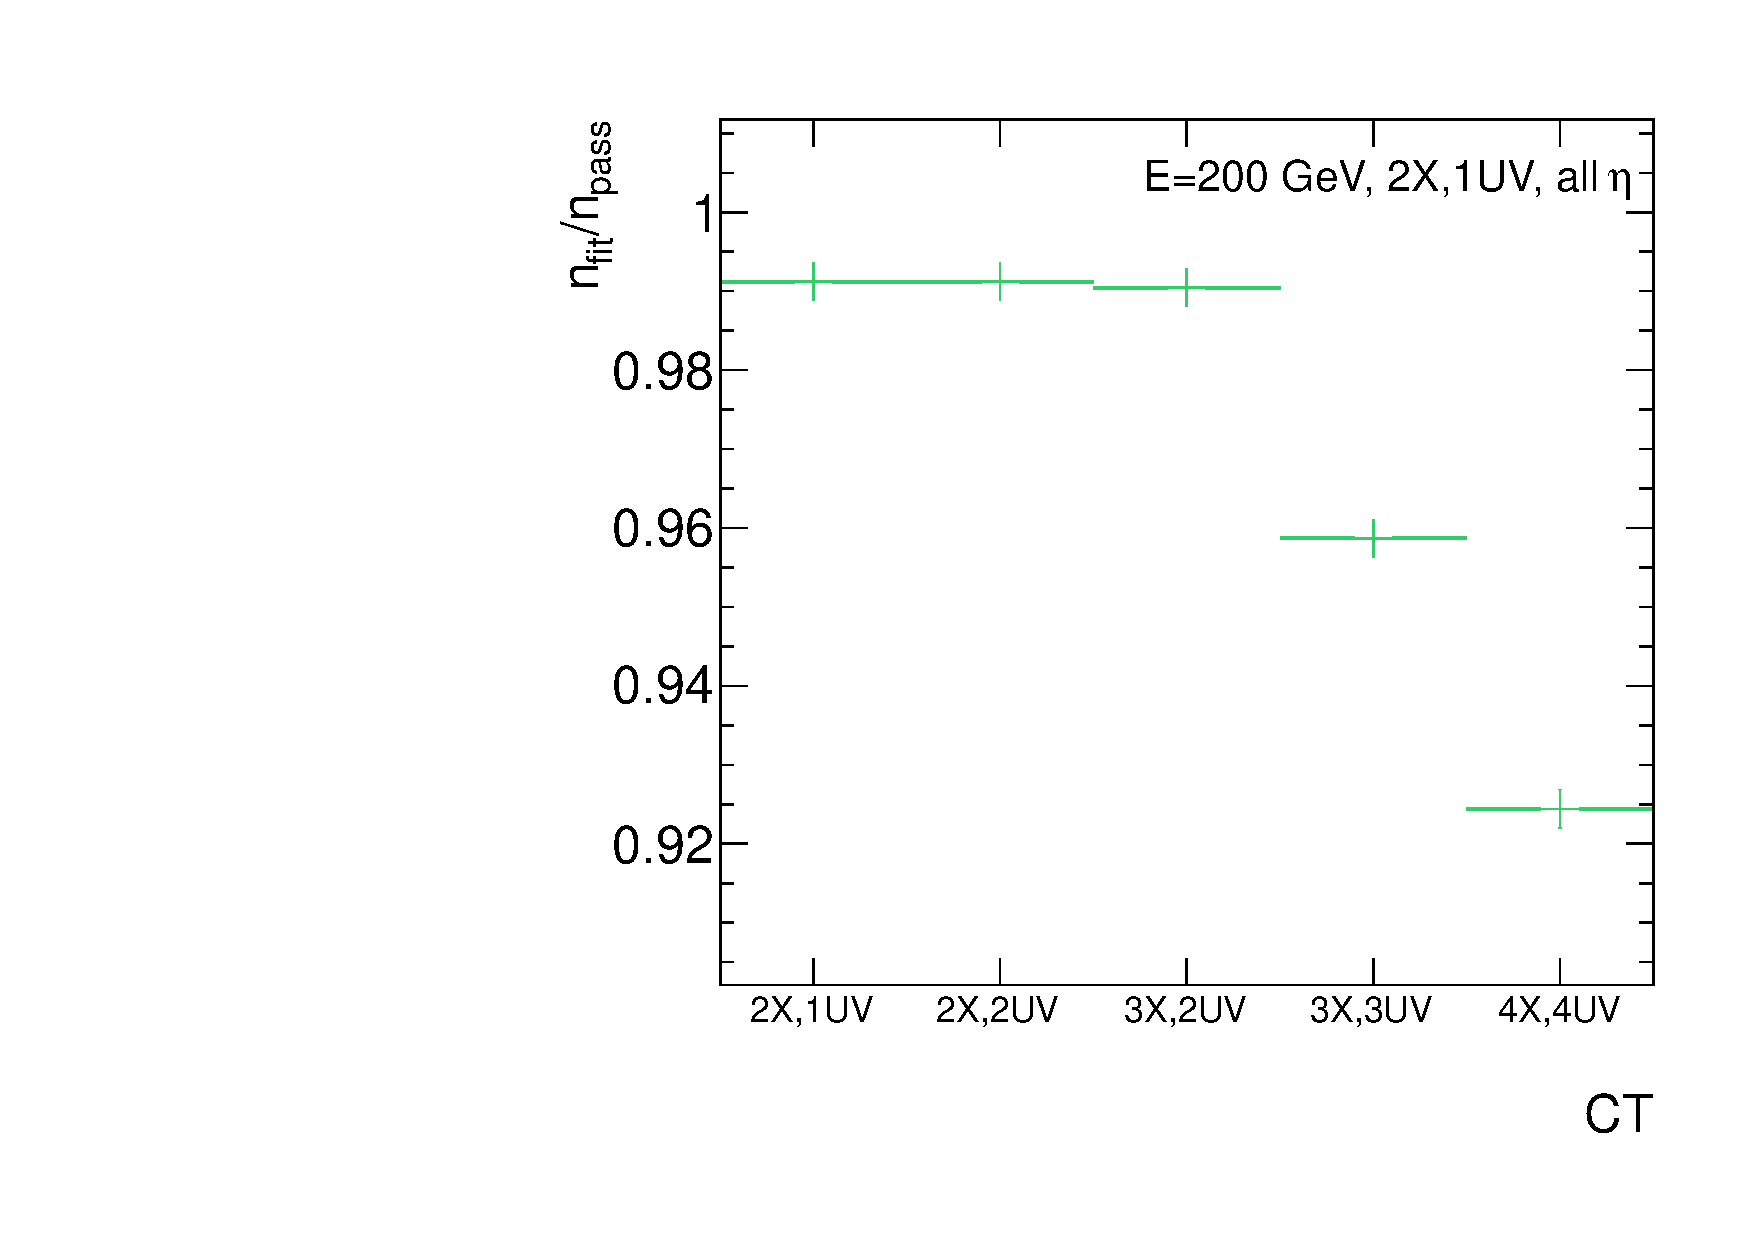
\includegraphics[width=0.33\textwidth]{algorithms-harvard/ct_var_2x_1uv_etaall_eff_6hit_200GeV.pdf}
	}
	\caption{\label{fig:harvard_ideal_eff}
Algorithmic efficiency~(a) showing for different coincidence thresholds (CT) at the truth trigger digit level,
the fraction of tracks that are fit. Total efficiency~(b) showing for different coincidence thresholds at the reconstructed
level, the fraction of total muons incident in the NSW surface that are fit with those thresholds. The efficiency for
different thresholds given that at least six hits are found at the truth level, as defined in Figure~\ref{fig:SaclayEfficiencyForDifferentPairRequirement} are shown in~(c).
	}
\end{figure}


The $\phi^{\rm{fit}}$, $\theta^{\rm{fit}}$ and $\Delta\theta^{\rm{fit}}$ resolutions for the ideal geometry for $E=200\GeV$ muons
without backgrounds, obtained from a fit are summarized in Table\,\ref{tab:efficiencyHarvardIdeal}. The efficiency, defined
as for Figure~\ref{fig:harvard_ideal_eff} (a) is also shown. 

\begin{table}[htbp]
\caption{Efficiency and resolution (mrad) for muons of $E=200\GeV$ for different coincidence thresholds without background.
\label{tab:efficiencyHarvardIdeal}  }
\centering
\begin{tabular}{l l c c c c}
\toprule
Track Type & Fit Efficiency & $\sigma(\theta^{\rm{fit}})$ (tails) & $\sigma(\phi^{\rm{fit}})$ (tails) & $\sigma(\Delta\theta^{\rm{fit}})$ (tails) \\ [0.5ex]
\midrule
4-horizontal/4-stereo & 99.8\% & 0.27 (0.83\%) & 2.3 (1.5\%) & 1.6 (0.65\%) \\
3-horizontal/3-stereo & 99.5\% & 0.28 (0.89\%) & 3.0 (0.97\%) & 1.7 (0.47\%)   \\
2-horizontal/2-stereo & 99.0\% & 0.29 (0.97\%) & 3.2 (1.1\%) & 1.9 (1.0\%)   \\
\bottomrule
\end{tabular}
\end{table}

\paragraph{Effects from incoherent background}  \hfill \\
The impact of backgrounds is studied in the geometry with perfect alignment.
Incoherent background extrapolated from measurements performed in Run\,1\cite{CERN-LHCC-2011-012}
is added outside of Athena to each generated event as hits after
the digitization step.  Background hits are uniformly distributed in $\phi$, and in time across two bunch
crossings (50\,ns).  Once generated for each event, the background hits are combined with true event hits and a VMM-mimicking
function is called by the simulation to choose only the earliest arrival hit for each VMM chip, which allows for the background to
sometimes mask a true trigger hit.

The $\phi^{\rm{fit}}$, $\theta^{\rm{fit}}$ and $\Delta\theta^{\rm{fit}}$ resolutions for the ideal geometry for E\,=\,200\,GeV muons
with backgrounds are summarized in Table\,\ref{tab:efficiencyHarvardBkg}. The efficiency, defined
as for Figure~\ref{fig:harvard_ideal_eff} (a) is also shown. 

\begin{table}[htbp]
\caption{Efficiency and resolution (mrad) for muons of $E=200\GeV$ for different coincidence thresholds with background.
\label{tab:efficiencyHarvardBkg}  }
\centering
\begin{tabular}{l l c c c c}
\toprule
Track Type & Fit Efficiency & $\sigma(\theta^{\rm{fit}})$ (tails) & $\sigma(\phi^{\rm{fit}})$ (tails) & $\sigma(\Delta\theta^{\rm{fit}})$ (tails) \\ [0.5ex]
\midrule
4-horizontal/4-stereo & 99.3\% & 0.30 (1.4\%) & 4.2 (1.5\%) & 1.7 (0.37\%) \\
3-horizontal/3-stereo & 99.0\% & 0.31 (1.9\%) & 4.8 (2.1\%) & 2.0 (0.58\%)   \\
2-horizontal/2-stereo & 98.2\% & 0.32 (2.0\%) & 5.1 (2.2\%) & 2.3 (0.82\%)   \\
\bottomrule
\end{tabular}
\end{table}

\paragraph{Effects from misalignments within the NSW}  \hfill \\
For the misalignments studied in this section, no changes in efficiency or in the
resolution of $\theta$ and $\phi$ have been
observed. However, a degradation in the resolution of the $\Delta\theta$ reconstruction
has been observed.

Figure\,\ref{fig:harvard_misal_effect} shows the relative change in $\Delta\theta^{\rm{fit}}$ resolution as a function of misalignment
for the different misalignment configurations illustrated in Figure\,\ref{fig:harvard_misal_illustration}.

\begin{figure}[htbp]
	\centering
	\subfloat[a][Shift in $r$]{
		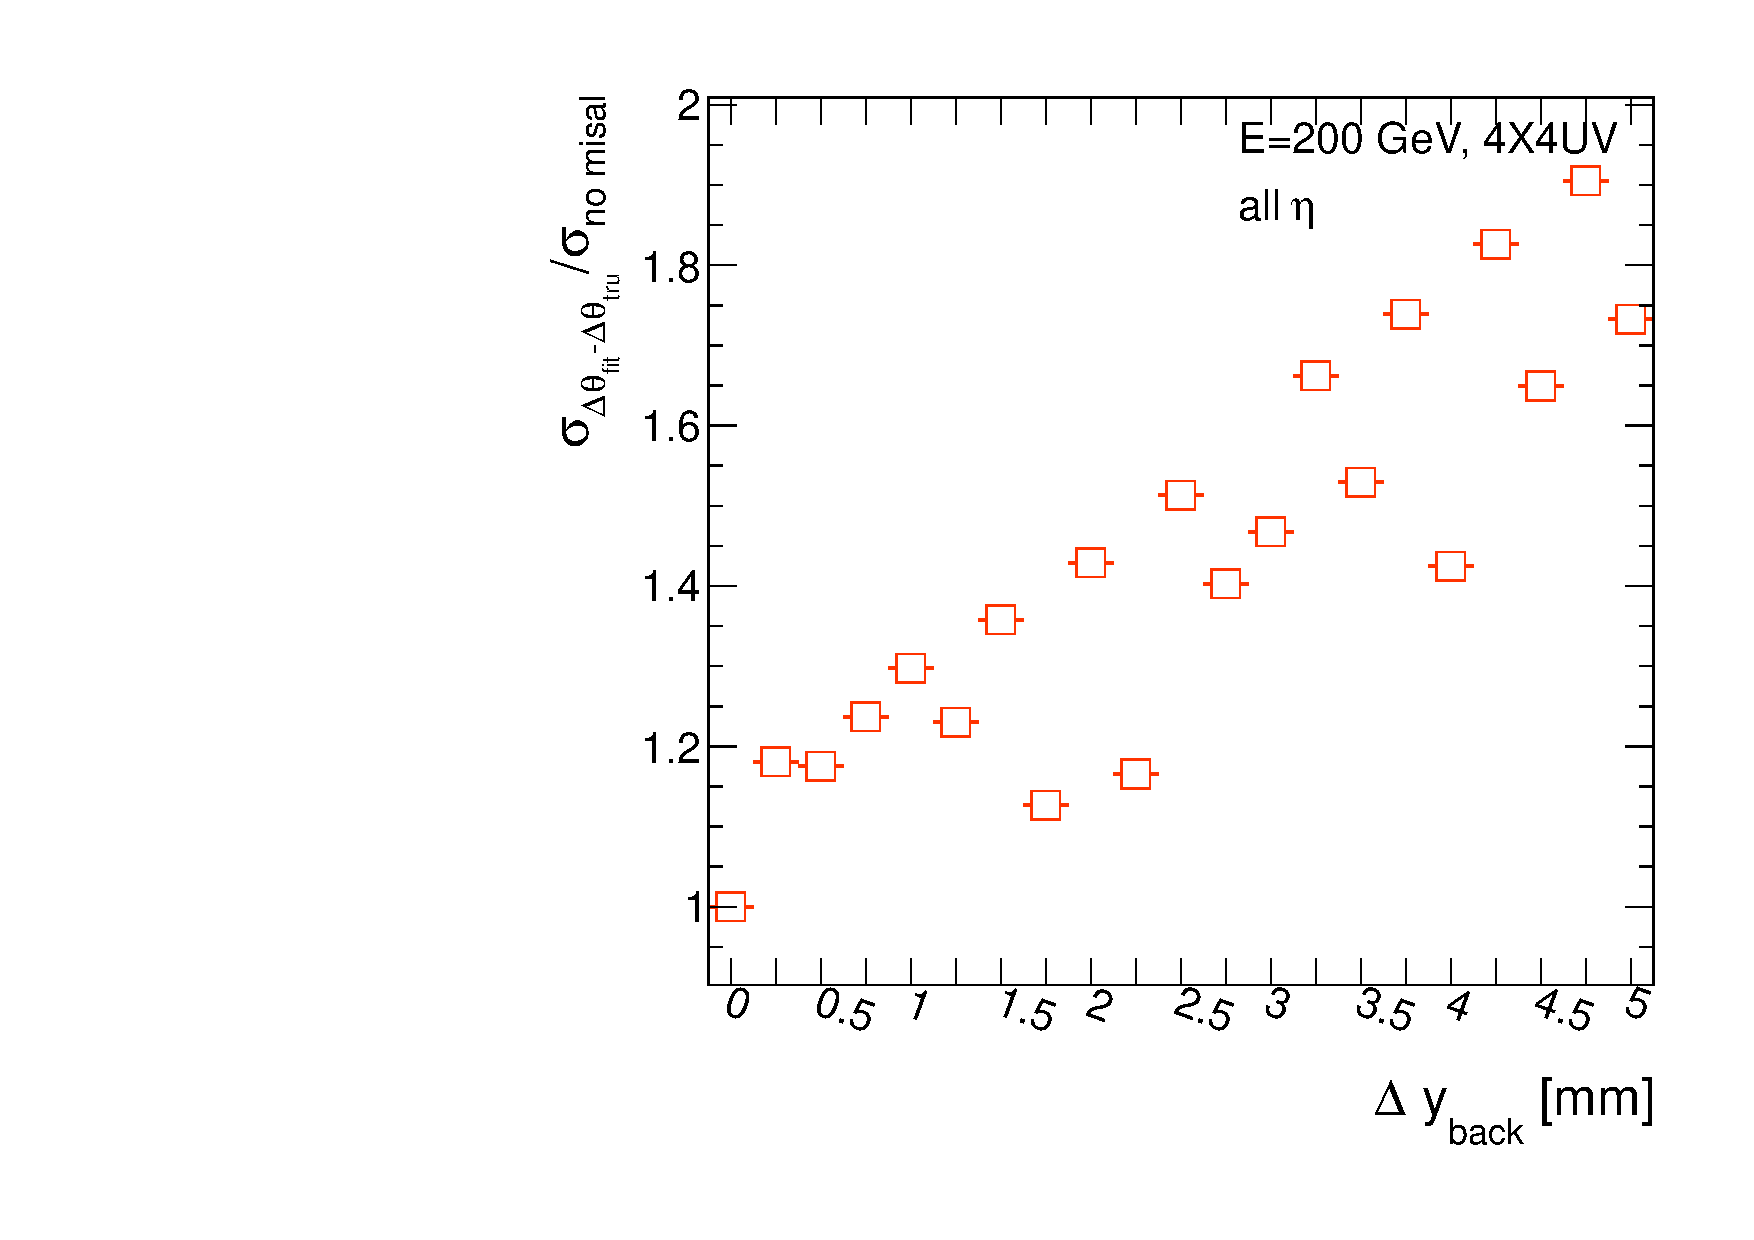
\includegraphics[width=0.32\textwidth]{algorithms-harvard/mmt_res_dtheta_misal_dyb_etaall_rel.pdf}
	}
	\subfloat[b][Top half shift in $r$]{
		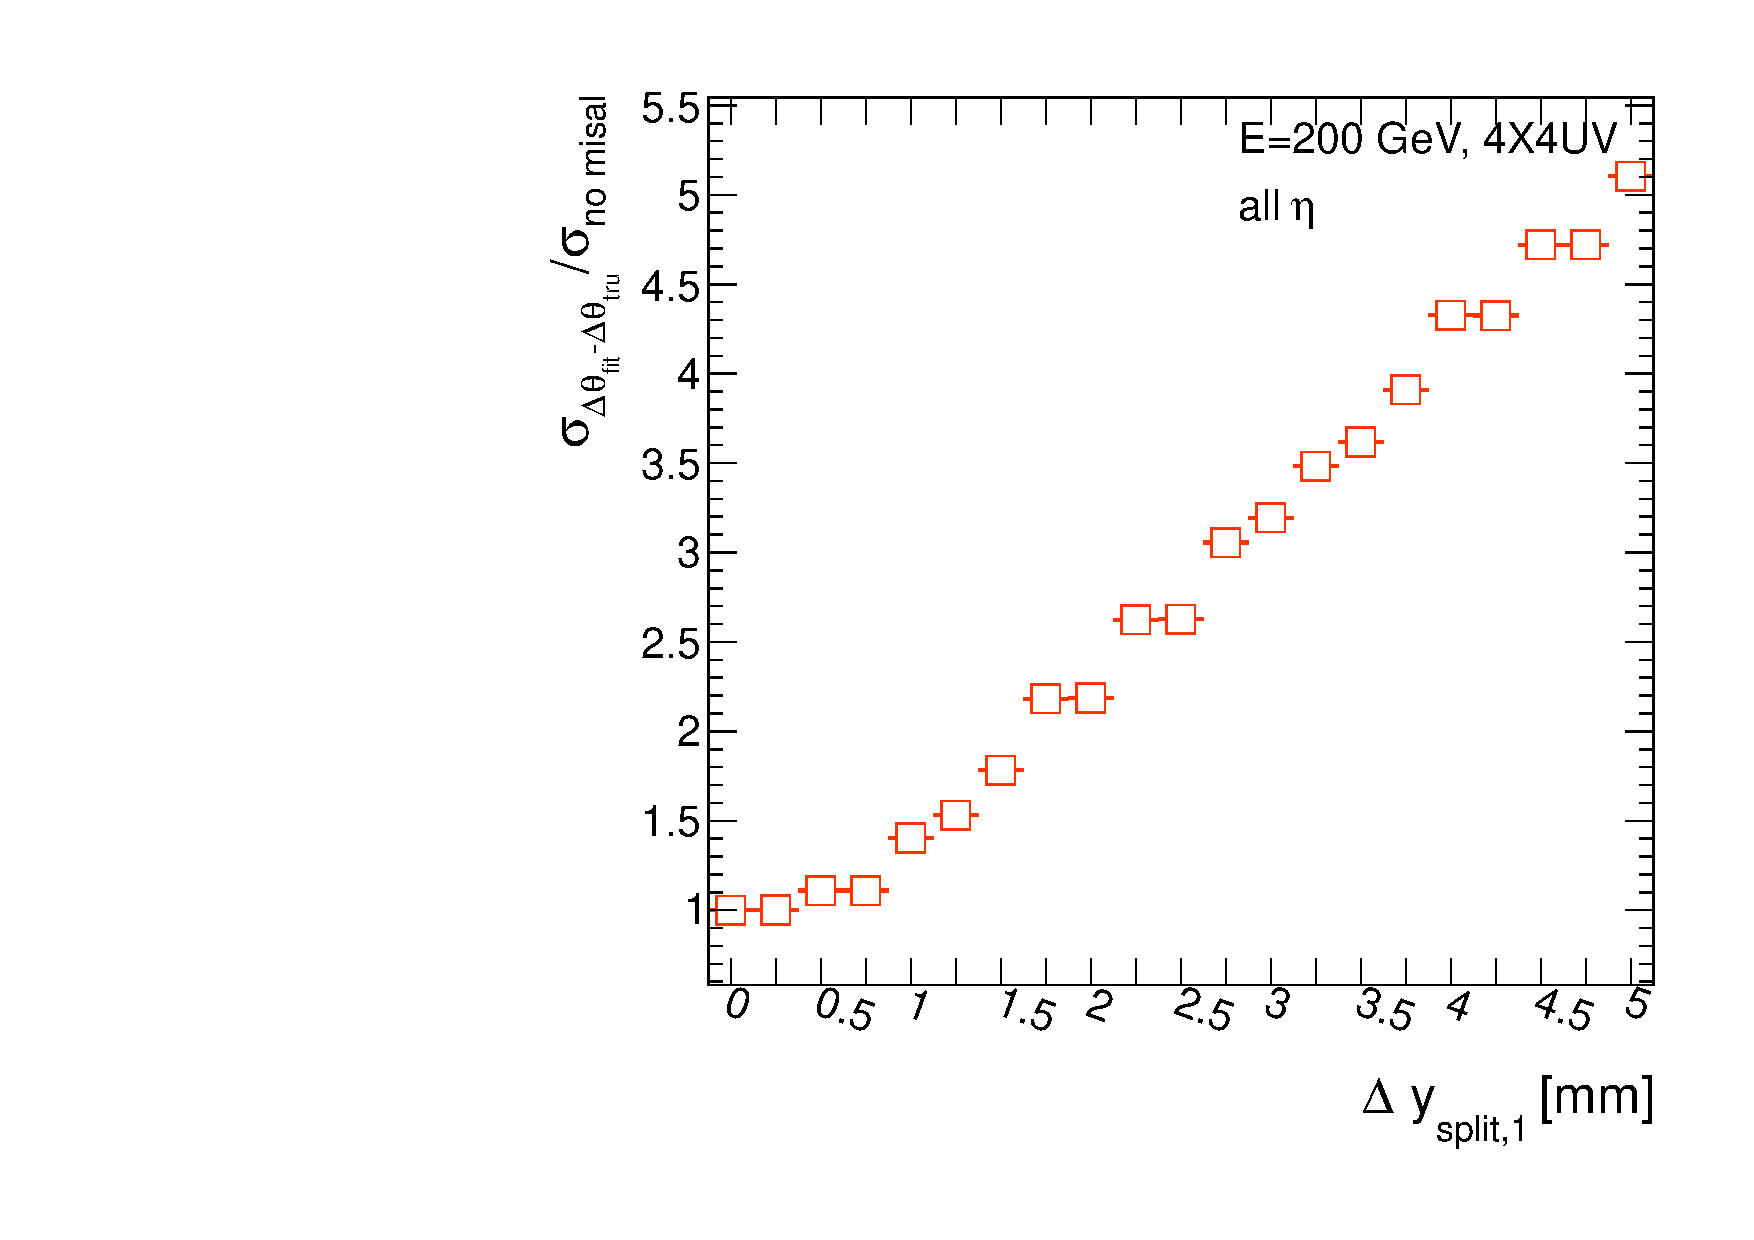
\includegraphics[width=0.32\textwidth]{algorithms-harvard/mmt_res_dtheta_misal_dyw1_etaall_rel.pdf}
	}
	\subfloat[c][$\phi$ rotation]{
		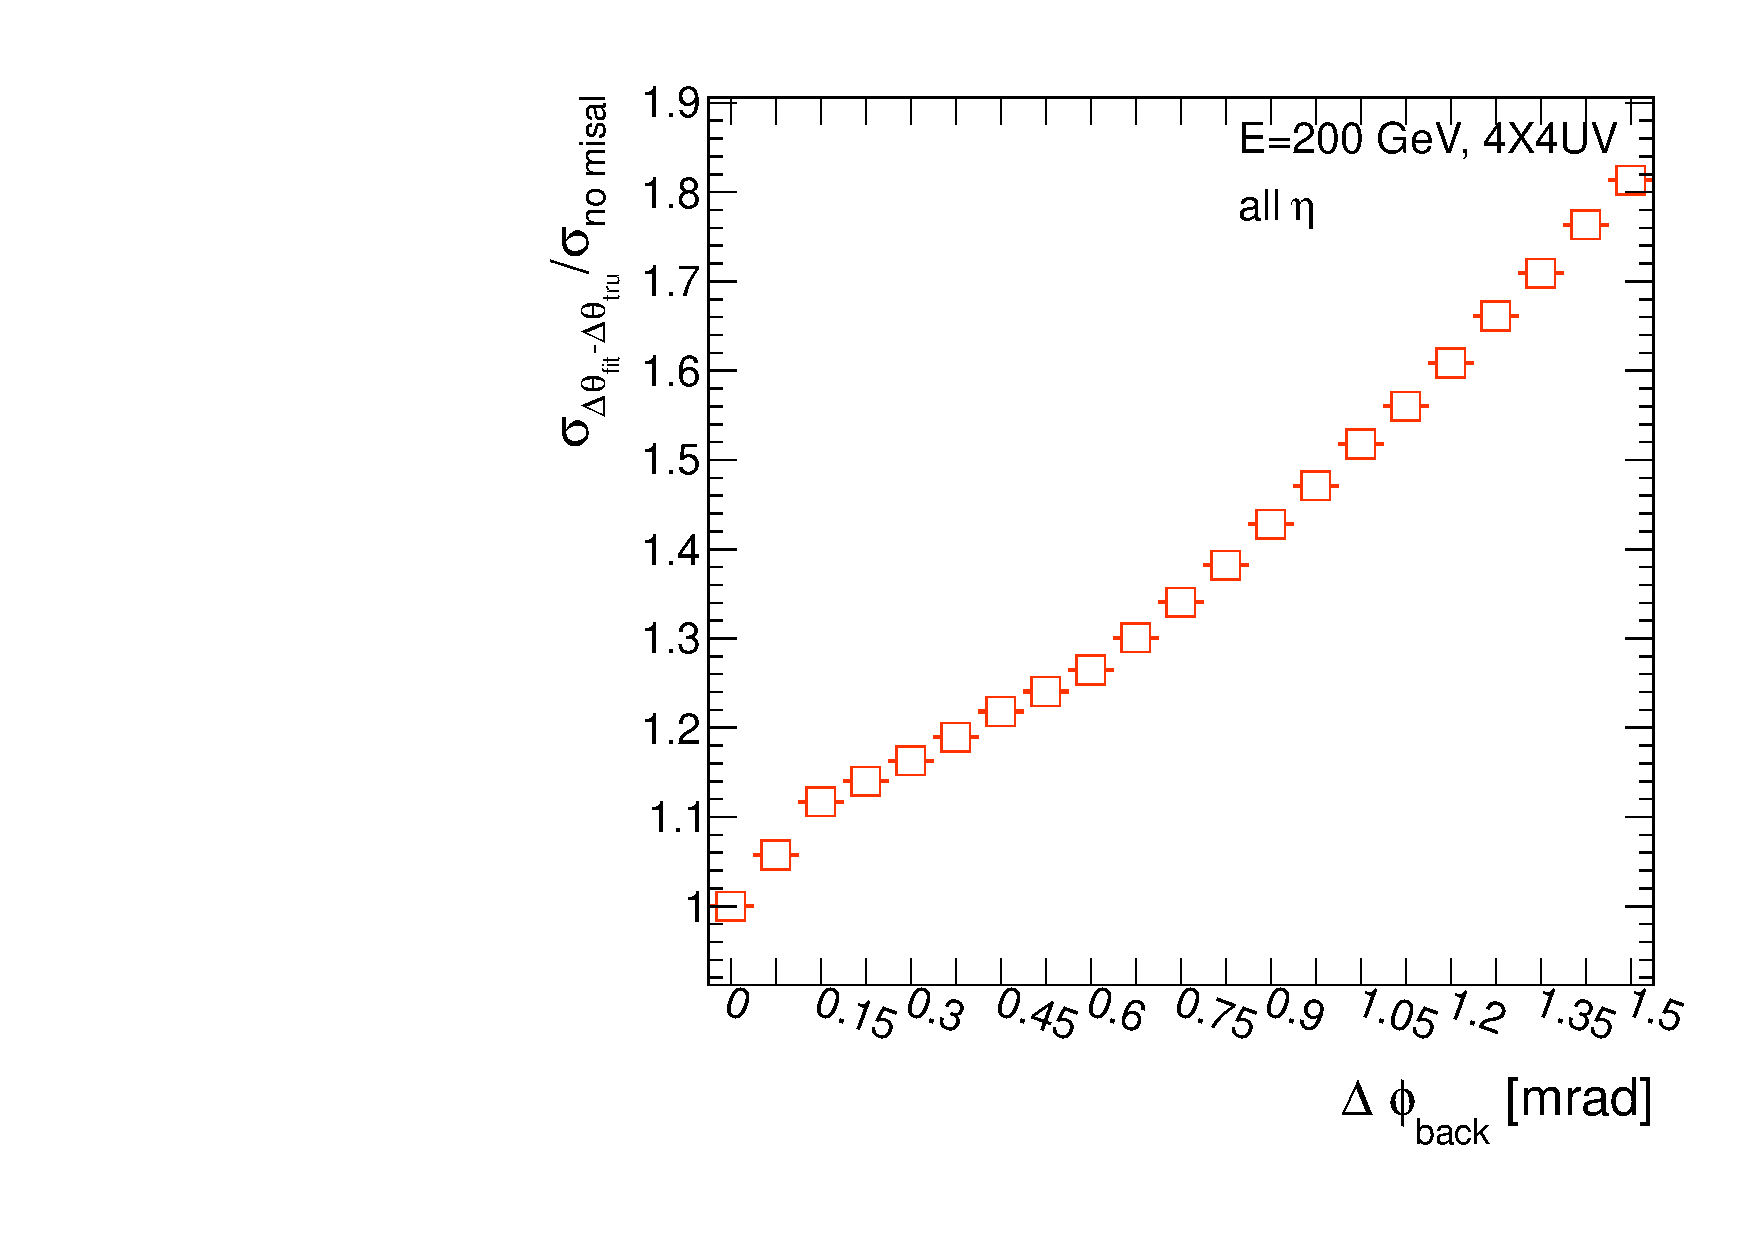
\includegraphics[width=0.32\textwidth]{algorithms-harvard/mmt_res_dtheta_misal_dpb_etaall_rel.pdf}
	}\\
	\subfloat[d][$\theta_{\rm tilt}$]{
		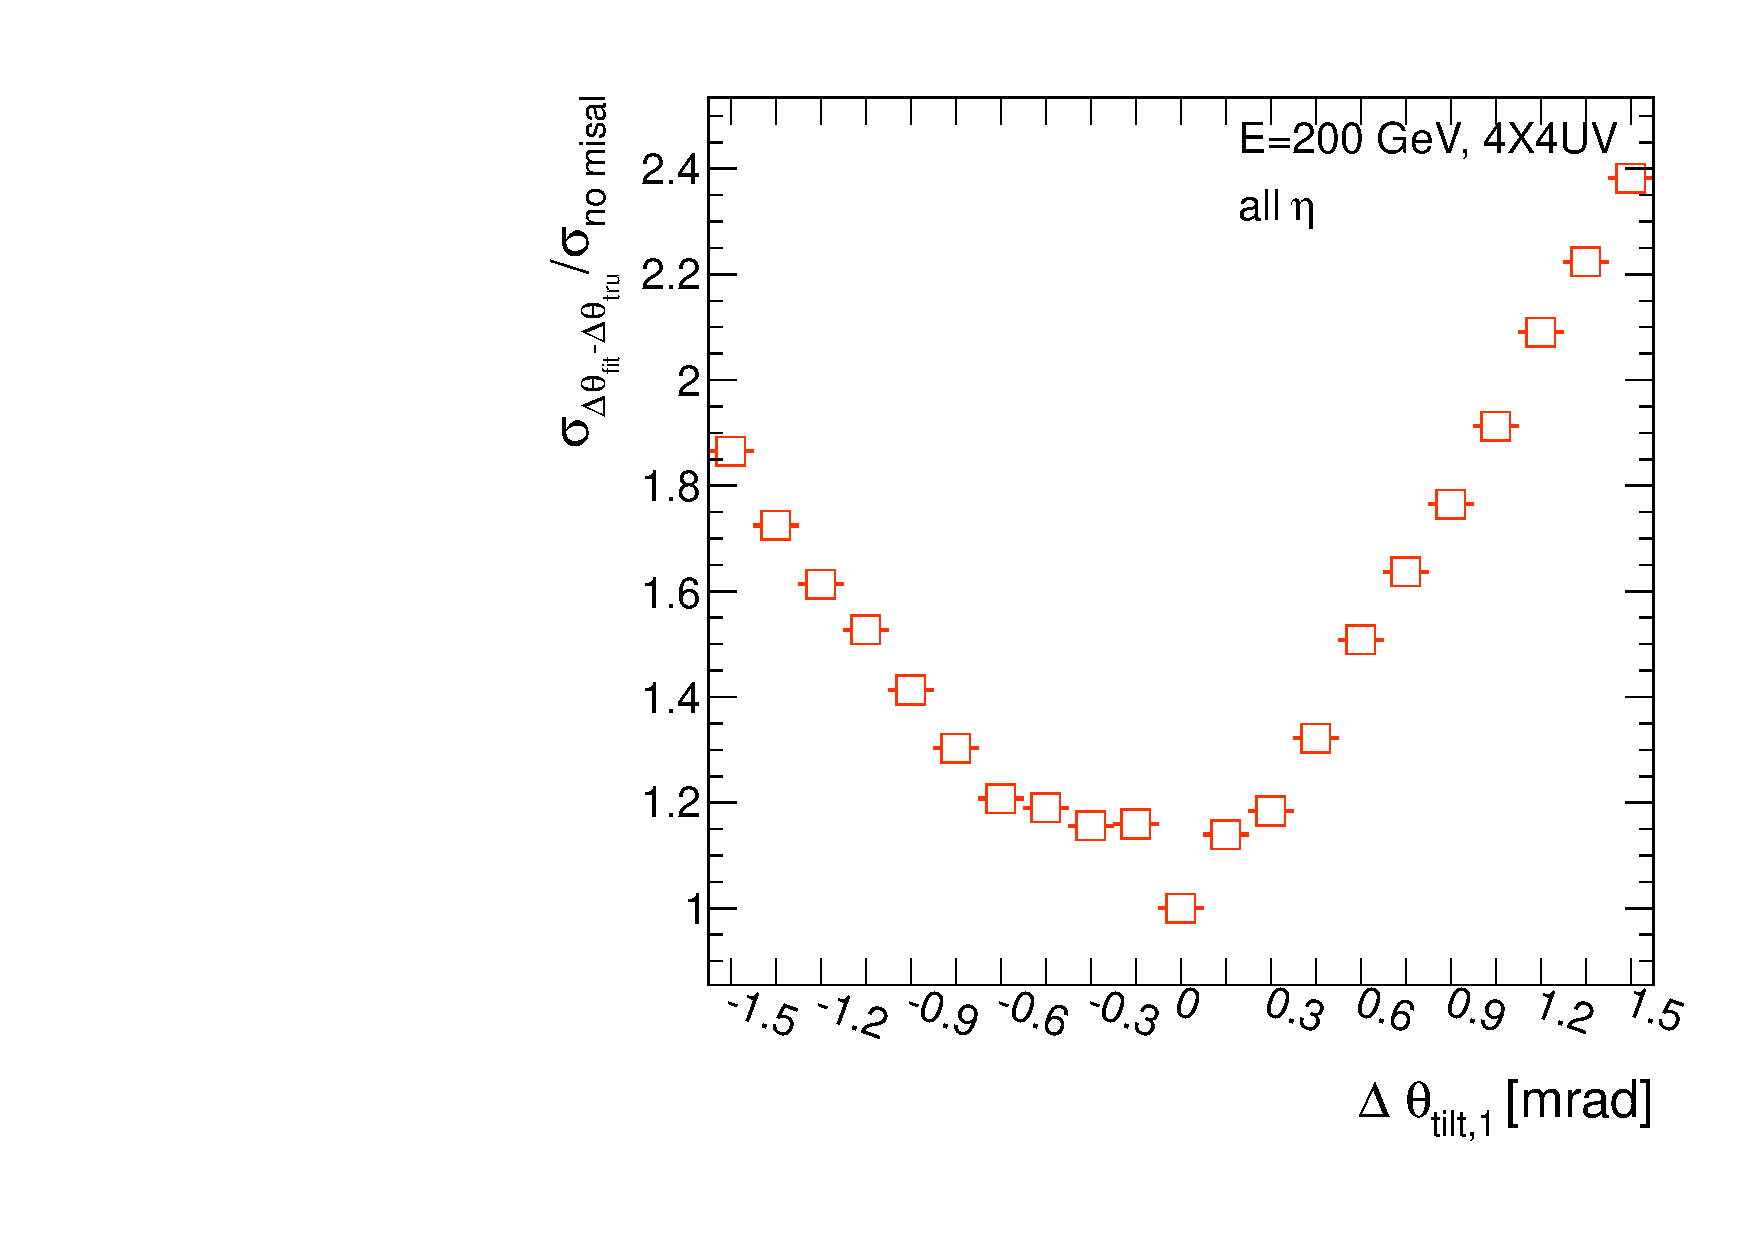
\includegraphics[width=0.32\textwidth]{algorithms-harvard/mmt_res_dtheta_misal_dt1_etaall_rel.pdf}
	}
	\subfloat[e][Shift in $z$]{
		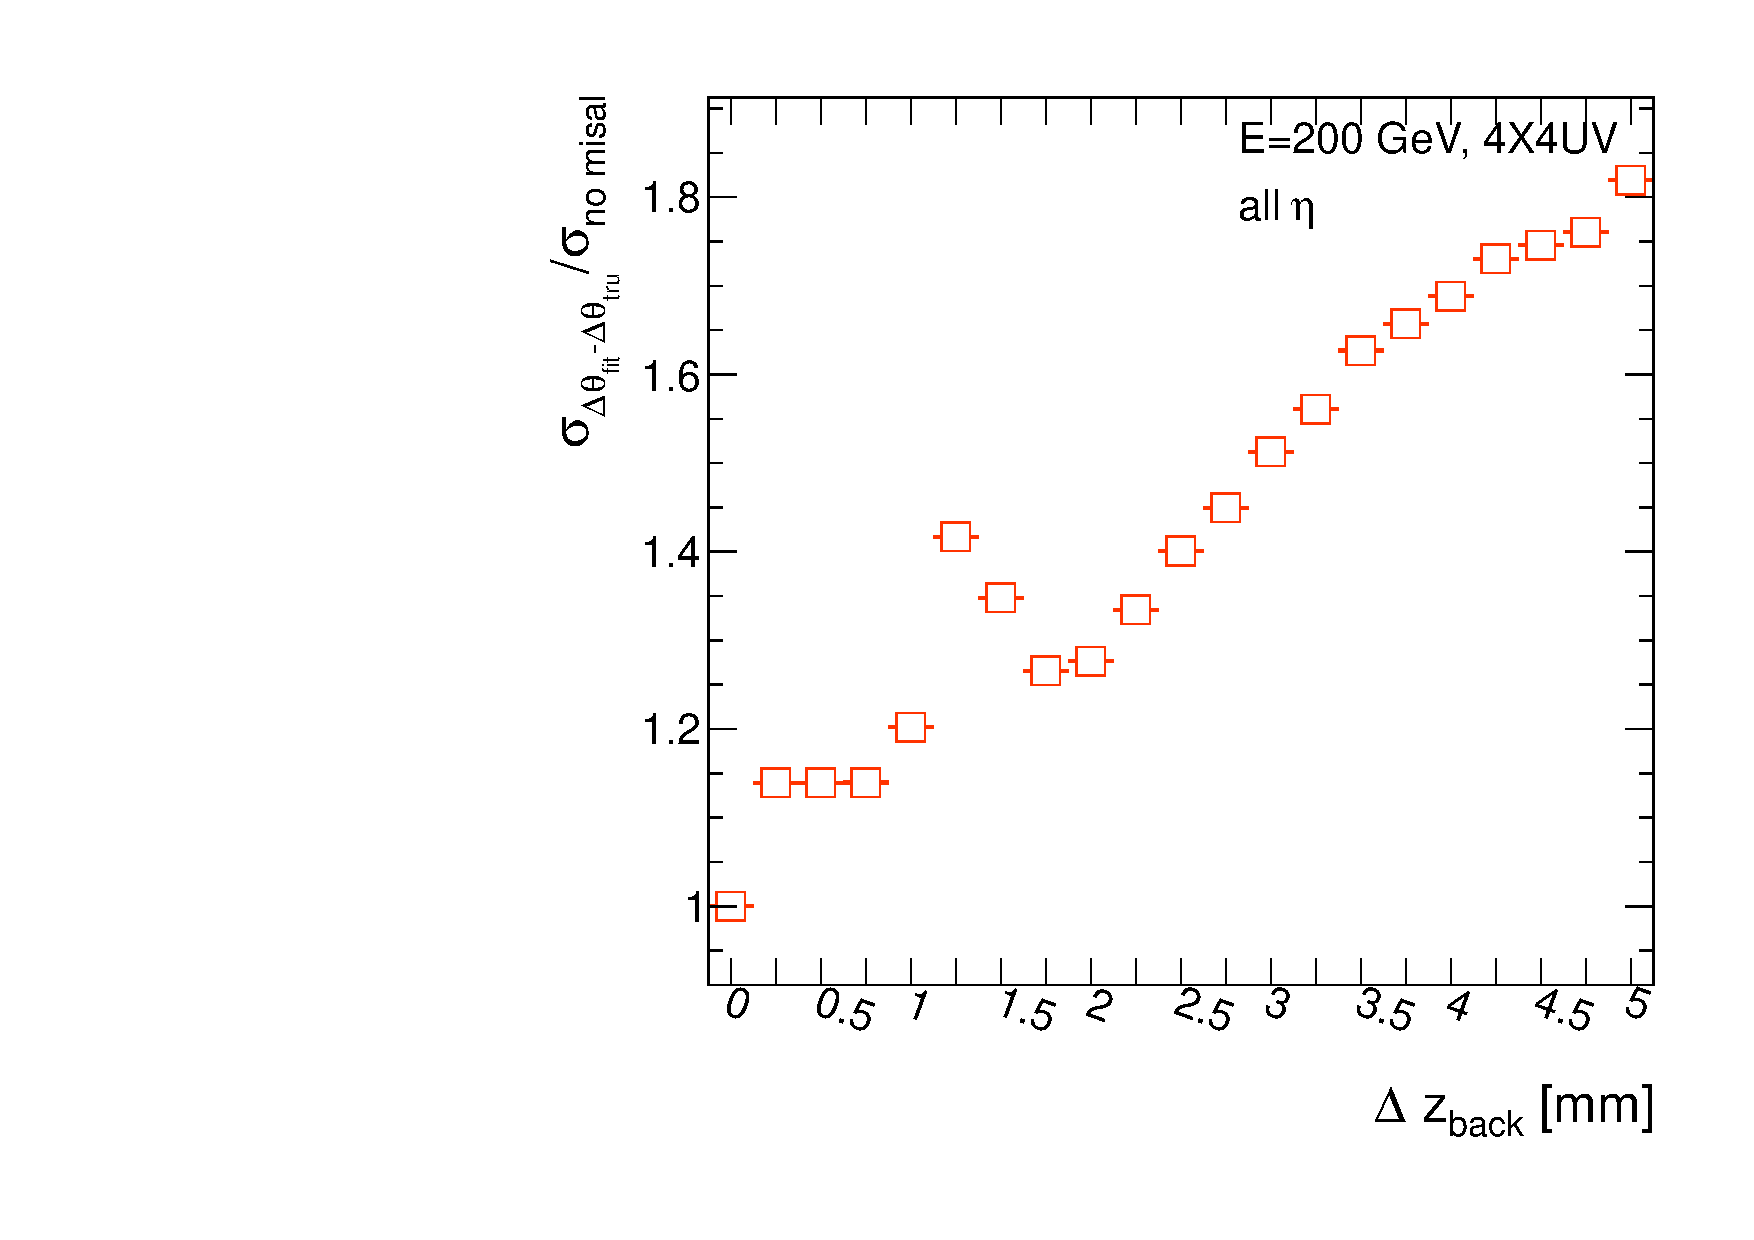
\includegraphics[width=0.32\textwidth]{algorithms-harvard/mmt_res_dtheta_misal_dzb_etaall_rel.pdf}
	}

	\caption{\label{fig:harvard_misal_effect}
	Relative change in $\Delta\theta^{\rm{fit}}$ resolution as a function of misalignment for different misalignment configurations.
	Figures (a)-(e) are laid out to match the corresponding misalignment as illustrated in Figure\,\ref{fig:harvard_misal_illustration}.
	}
\end{figure}

The degradation shows a certain periodicity related to strip width for displacements. This is clear for
Figures\,\ref{fig:harvard_misal_effect}\,(a) and~(b). The degradation is higher when only half of the
detector is radially shifted (b) because a double peak structure is formed, which increases more significantly
the peak width. Rotations (c and d) cause monotonic changes in performance. The degradation is more
significant when the tilt is away from the IP (positive axis) because more strips are forced to cover the same
solid angle, increasing the effective distance between the strip that should have been hit and the strip that
is actually hit. Figure\,\ref{fig:harvard_misal_effect}\,(e) shows at lower levels of misalignment a fixed level of degradation, again
caused by a discrete strip width. At around 1\,mm a two-peak structure appears in the distribution, which causes
an increase in the RMS. As the distribution gets further smeared the double peak structure disappears, yielding
a monotonically increasing degradation. Additional results can be found in Ref.~\cite{harvard-alg-misal}.

%These results are summarized in Table~\ref{tab:harv-misal}.
%\begin{table}
  %\centering
  %\begin{tabular}{|c|l|l|l|l|l|}%p{4.5cm}|}
    %\hline
    %Type          & $\Delta y_{back}$ & $\Delta y_{top}$ & $\Delta z_{back}$ & $\Delta\phi_{back}$ & $\Delta\theta_{tilt}$\\
    %\hline
   % Range studied &    0--5 mm        &   0--5 mm        &    0--5 mm        &    0--1.5 mrad      &    -1.5--+1.5 mrad   \\
    %\hline
    %25\%          &    0.75 mm        &     0.5 mm       &    1.25 mm        &       0.6 mrad      &    (-0.9)+0.45 mrad   \\
    %50\%          &     2.5 mm        &    1.25 mm       &     3.0 mm        &      1.05 mrad       &   (-1.05)+0.75 mrad   \\
    %\hline
   % Remarks       & \multicolumn{2}{|c|}{periodic in $w_{strip}$} & peak from geo. eff. & mono. inc. & +(-) is (away) twds. IP\\
    %\hline
  %\end{tabular}
  %\caption{\label{tab:harv-misal} Increase of resolution on $\Delta\theta$ error summary; levels of misalignment corresponding to \% increases in resolution are quoted.}
%\end{table}

It should be noted that corrections for all cases, except (c) have been developed. Based on these current
corrections, since only case (c) is relevant, a degradation
of up to 75\% on $\Delta\theta^{\rm{fit}}$ resolution (or from 1.7\,mrad to 3.0\,mrad in the 4-horizontal/4-stereo case) is
expected for 5\,mm misalignments.

\paragraph{Performance with the xxuv uvxx configuration}  \hfill \\
Recently, it has been decided to build sectors with the mirror-image placement (resulting
in a xxuv uvxx horizontal/stereo strip configuration). From the perspective of
the trigger, new simulations have not been produced yet. However, estimates of the improvement
in the $\Delta\theta^{\rm{fit}}$ resolution have been obtained\cite{harvard-alg-xxuvuvxx}.

The estimate has been performed using a
toy simulation of the trigger algorithm, which does not include any ionization or scattering effects.
This simulation only demonstrates resolution effects arising from the width of the strips. Based
on this simulation, an ideal geometrical $\Delta\theta^{\rm{fit}}$ resolution of 0.89\,mrad has been estimated for the
4-horizontal/4-stereo hit category in the standard geometry. This number can be used together
with the resolution obtained in the full simulation (and shown in Table\,\ref{tab:efficiencyHarvardIdeal})
to estimate the impact of different physics effects (ionization, multiple scattering...)
in the resolution. In particular, using $\sigma_{\rm athena}^2=\sigma_{\rm physics}^2+\sigma_{\rm geometry}^2$,
one can estimate $\sigma_{\rm physics}$. The toy simulation can then be used to calculate the new
$\sigma^{\rm new}_{\rm geometry}=0.79$ for the mirror-image geometry. This, combined with $\sigma_{\rm physics}$
provides the estimate of the quantity of interest $\sigma^{\rm new}_{\rm athena}$. Using this procedure,
one estimates that with the new geometry the ideal $\Delta\theta^{\rm{fit}}$ resolution for the 4-horizontal/4-stereo
hit category improves to 1.65\,mrad from 1.7\,mrad, or less than 5\%, in the case with backgrounds.
These studies are reported in more
detail in Ref.\,\cite{harvard-alg-xxuvuvxx} and need to be repeated using the ATLAS full simulation.

\subsubsubsection{Summary} 
An algorithm for the reconstruction of segments using trigger hits in the MM detector has been described. 
The algorithm has been tested using events passed through the ATLAS full simulation with a realistic detector geometry and 
description of the signal formation. The algorithm presented has a very high efficiency of close to 100\%, a 
position resolution
in $\theta$ and $\phi$ of $\approx 0.3$~mrad and $\approx 3$~mrad, respectively, and a $\Delta\theta$ resolution of 
$\approx 1.7$~mrad. The algorithm has also been tested in conditions including incoherent background at realistic rates, showing
very comparable performance, except on the $\phi$ resolution, which degrades to $\approx 5$~mrad. 
To achieve high efficiency, relatively loose requirements on the number of hits (2 horizontal strips and one stereo
strip) need to be imposed. Tighter requirements, which might prove necessary to reject backgrounds, can be applied. A requirement
of 3 horizontal and 3 stereo strip hits yields an efficiency of about 92\%. 

The algorithm has been implemented in a Virtex XC7VX485T FPGA and its latency has been estimated with this
set-up at 56\,ns for the current implementation, using a 320~MHz clock. Memory resources have also been
estimated using this set up and fall well within the capabilities of this FPGA with a 30\% margin. This simulation
does not include some additional functionality, such as misalignment corrections or ancillary functions, so the
possibility of using a pin-compatible FPGA with higher resources is currently being investigated. 

Misalignment conditions have been simulated using truth hit information from the ATLAS full simulation. Misalignments of
up to 5\,mm have been considered. No significant changes in algorithmic efficiency, $\phi$ or $\theta$ resolution have 
been observed. The reconstruction of $\Delta\theta$ is affected by these misalignments. In particular, a significant
degradation of the resolution has been observed. Corrections requiring low resources in the FPGA have been 
described for four out of the five types of misalignments surveyed. For the fifth type, corrections can be designed, 
but they would increase the latency of the algorithm and their impact on the overall resources needs to be studied. 
Estimates have been provided for the degradation in the $\Delta\theta$ resolution for this case of at most 75\%, resulting
in a resolution of 3.0\,mrad for sectors with local misalignments of 5\,mm. 
